
In the signal region, events consist of 1 lepton, at least 4 jets, and \MET. The QCD multijet 
events contain only jets at parton level. However, after event reconstruction, these events can 
still have leptons from the misidentifications of light jets, and \MET due to the poor measurement of 
energy in the detector. The leptons can also be produced from the decay of bottom and charm hadrons. 
The \MET can also arise due to the mismeasurement of hadronic activity inside the CMS detector. 
Having the same event topology as that of signal, the QCD multijet process is also considered as a 
background for this analysis. However, it contributes only around 2\% of the total backgrounds.

The simulation of QCD multijet events are CPU time consuming due to which we can not generate them 
in large numbers due to computing limitations. Due to the lesser number of events, 
compared to the cross section, the statistical uncertainty is high. Also, the simulated events 
are not properly modeled for high jet multiplicities. After lepton trigger selection, the relative 
isolation plots from data and simulated events are shown in Figures~\ref{subfig:RelIso_mu},
\ref{subfig:RelIso_ele} for \mujets and \ejets channel, respectively. From these figures, 
it is obvious that the events with $I_{\text{rel}}^{\mu} \geq 0.20$ and $I_{\text{rel}}^{e} \geq 0.10$
are dominated by QCD multijet processes. However, there is a poor agreement between data and simulation
for $I_{\text{rel}}^{\mu} > 0.20$ and $I_{\text{rel}}^{e} > 0.10$ for both \mujets and \ejets channel.
In view of the above, the QCD multijet background is estimated from data to have a precise estimation. 

To estimate QCD multijet events from data, a method similar to the ABCD method is followed. The 
ABCD region, as shown in Figure~\ref{fig:abcd}, is formed from two uncorrelated variables, \MET 
and $I_{\text{rel}}$ (relative isolation as defined in Equations (\ref{eq:mu_iso}) and (\ref{eq:ele_iso})). 
The correlation between \MET and $I_{\text{rel}}$ are shown in 
Figures~\ref{subfig:RelIso_MET_TProf_muData} (\ref{subfig:RelIso_MET_TProf_eleData}),
\ref{subfig:RelIso_MET_TProf_muQCD} (\ref{subfig:RelIso_MET_TProf_eleQCD}) from data and simulated 
QCD multijet process for \mujets (\ejets) channel. The comparison between data and simulation for \MET 
and $I_{\text{rel}}$  are shown in Figure~\ref{fig:qcdVar} after 1-lepton selection, of 
Section~\ref{s:secEvtSel}, for \mujets and \ejets channel. From this figure, it can be 
seen that the QCD multijet process is dominated in high $I_{\text{rel}}$ region. The signal region 
lies in high \MET and low $I_{\text{rel}}$ (region-A of Figure~\ref{fig:abcd}). We estimate QCD 
multijet in the region-A from other regions as described in the following sections.

\begin{figure}
    \centering  
    \subfigure[\label{subfig:RelIso_mu}]
    {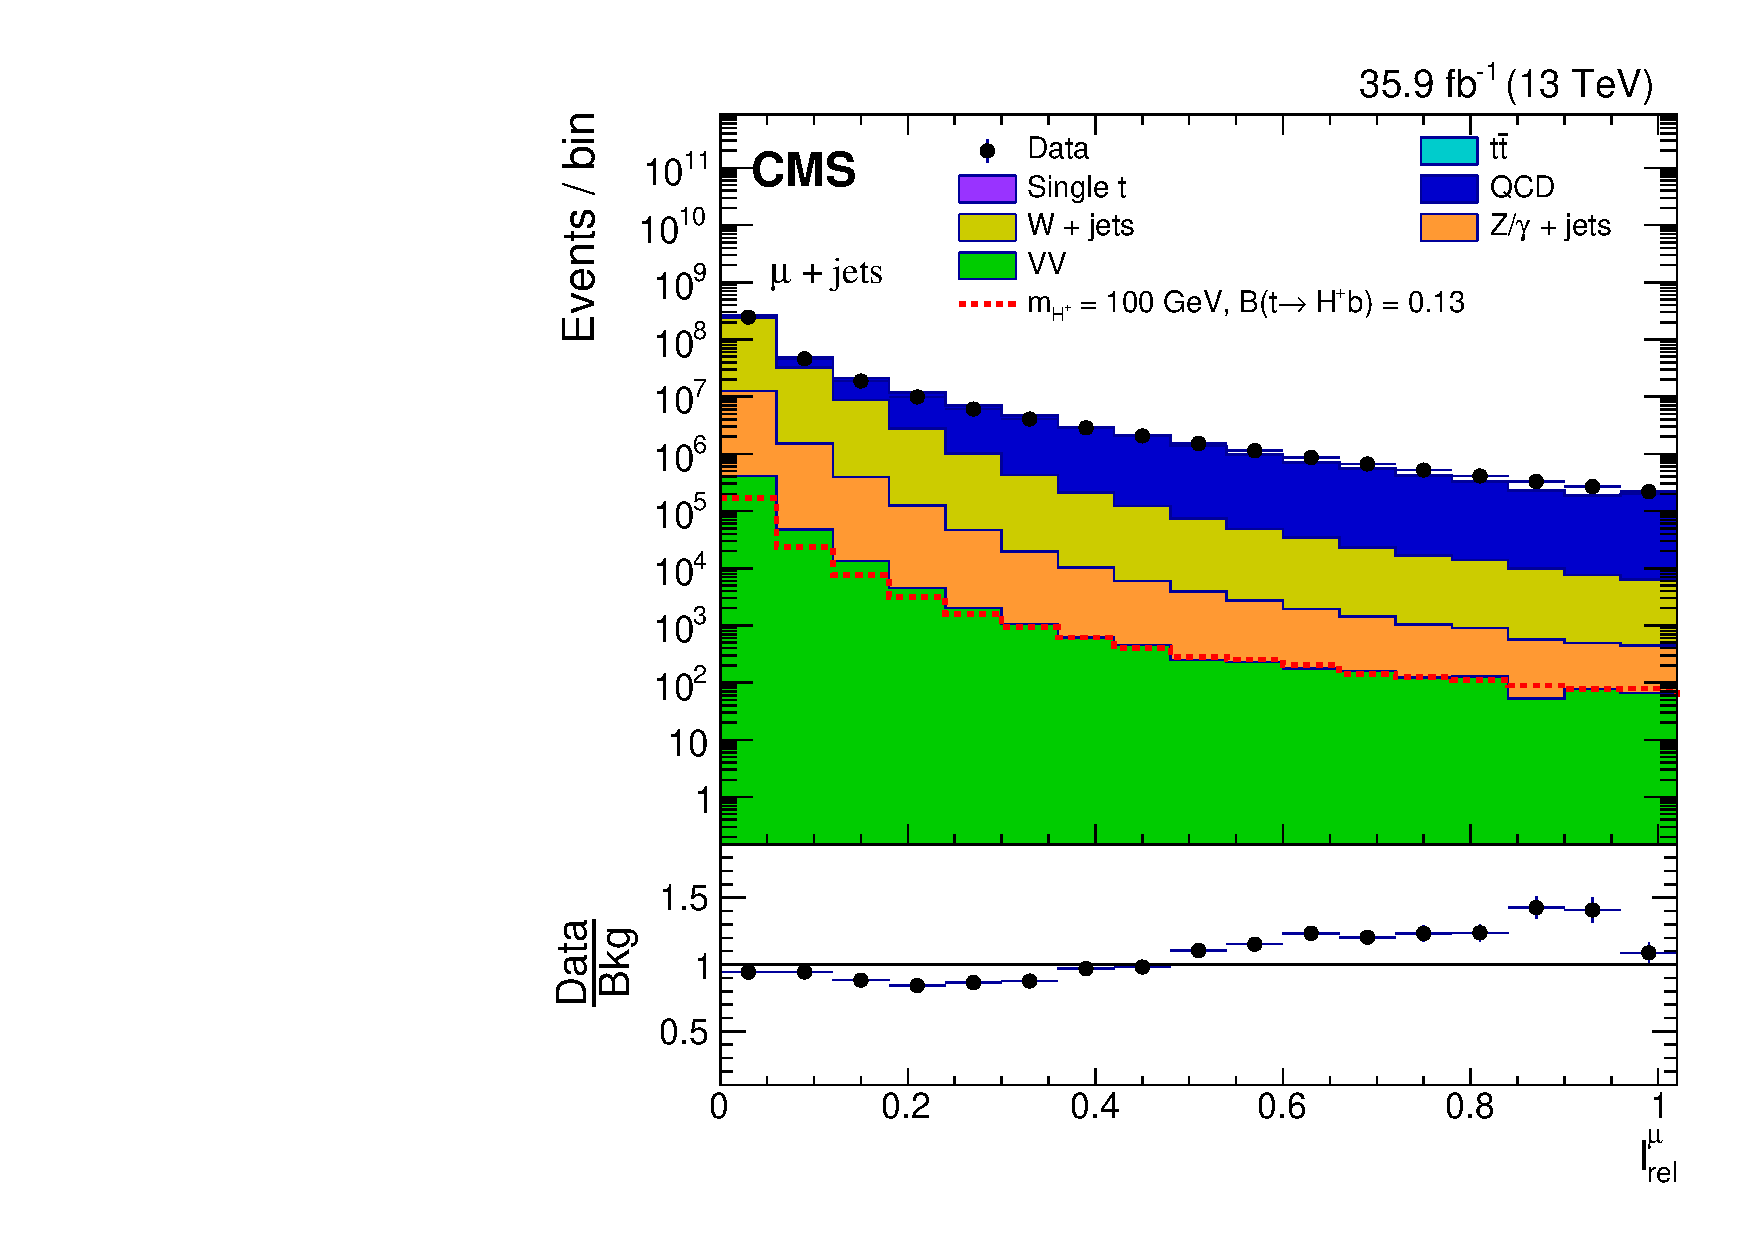
\includegraphics[width=0.49\linewidth]{Image/Muon/RelIso_1Mu_mu.pdf}}
    \subfigure[\label{subfig:RelIso_ele} ]
    {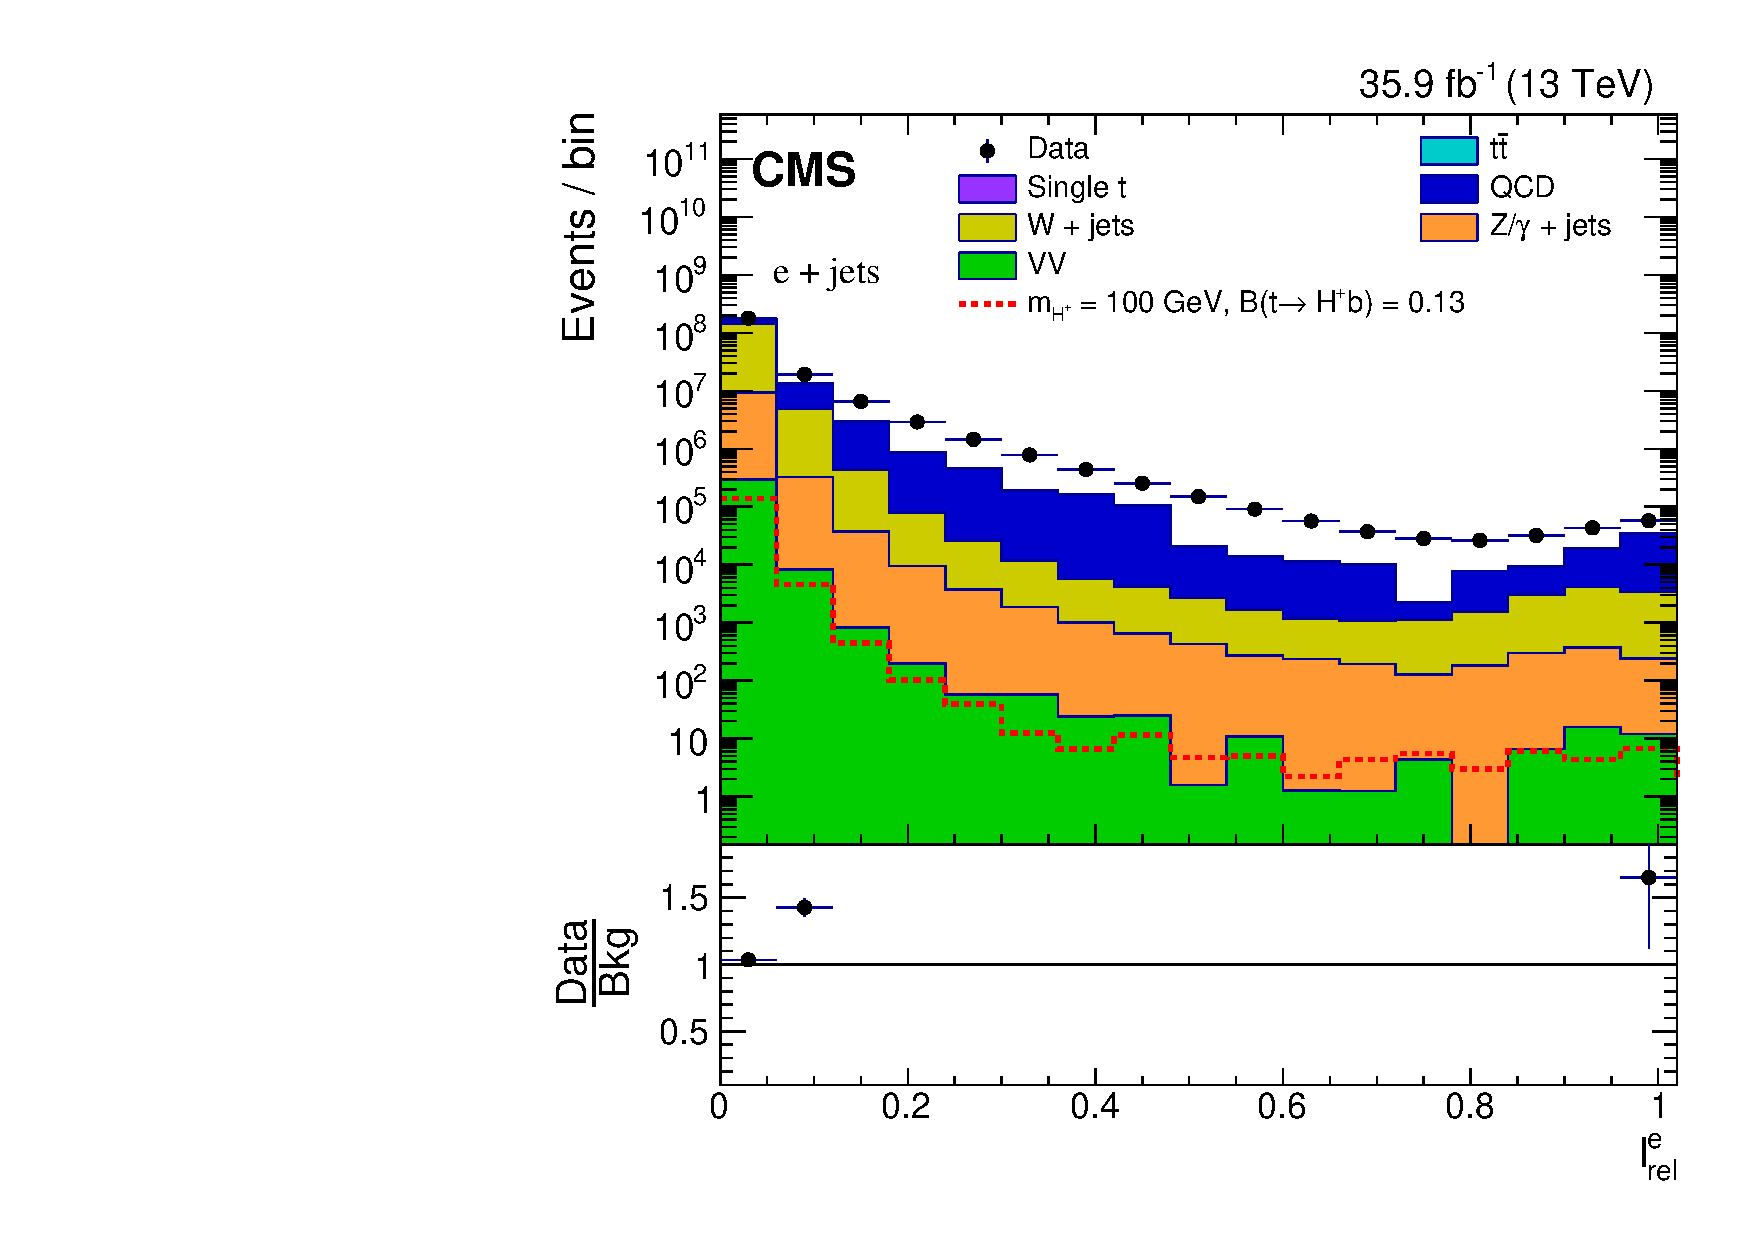
\includegraphics[width=0.49\linewidth]{Image/Electron/RelIso_1Ele_ele.pdf}}
    \vfil
    \subfigure[\label{subfig:pt_met_mu}]
    {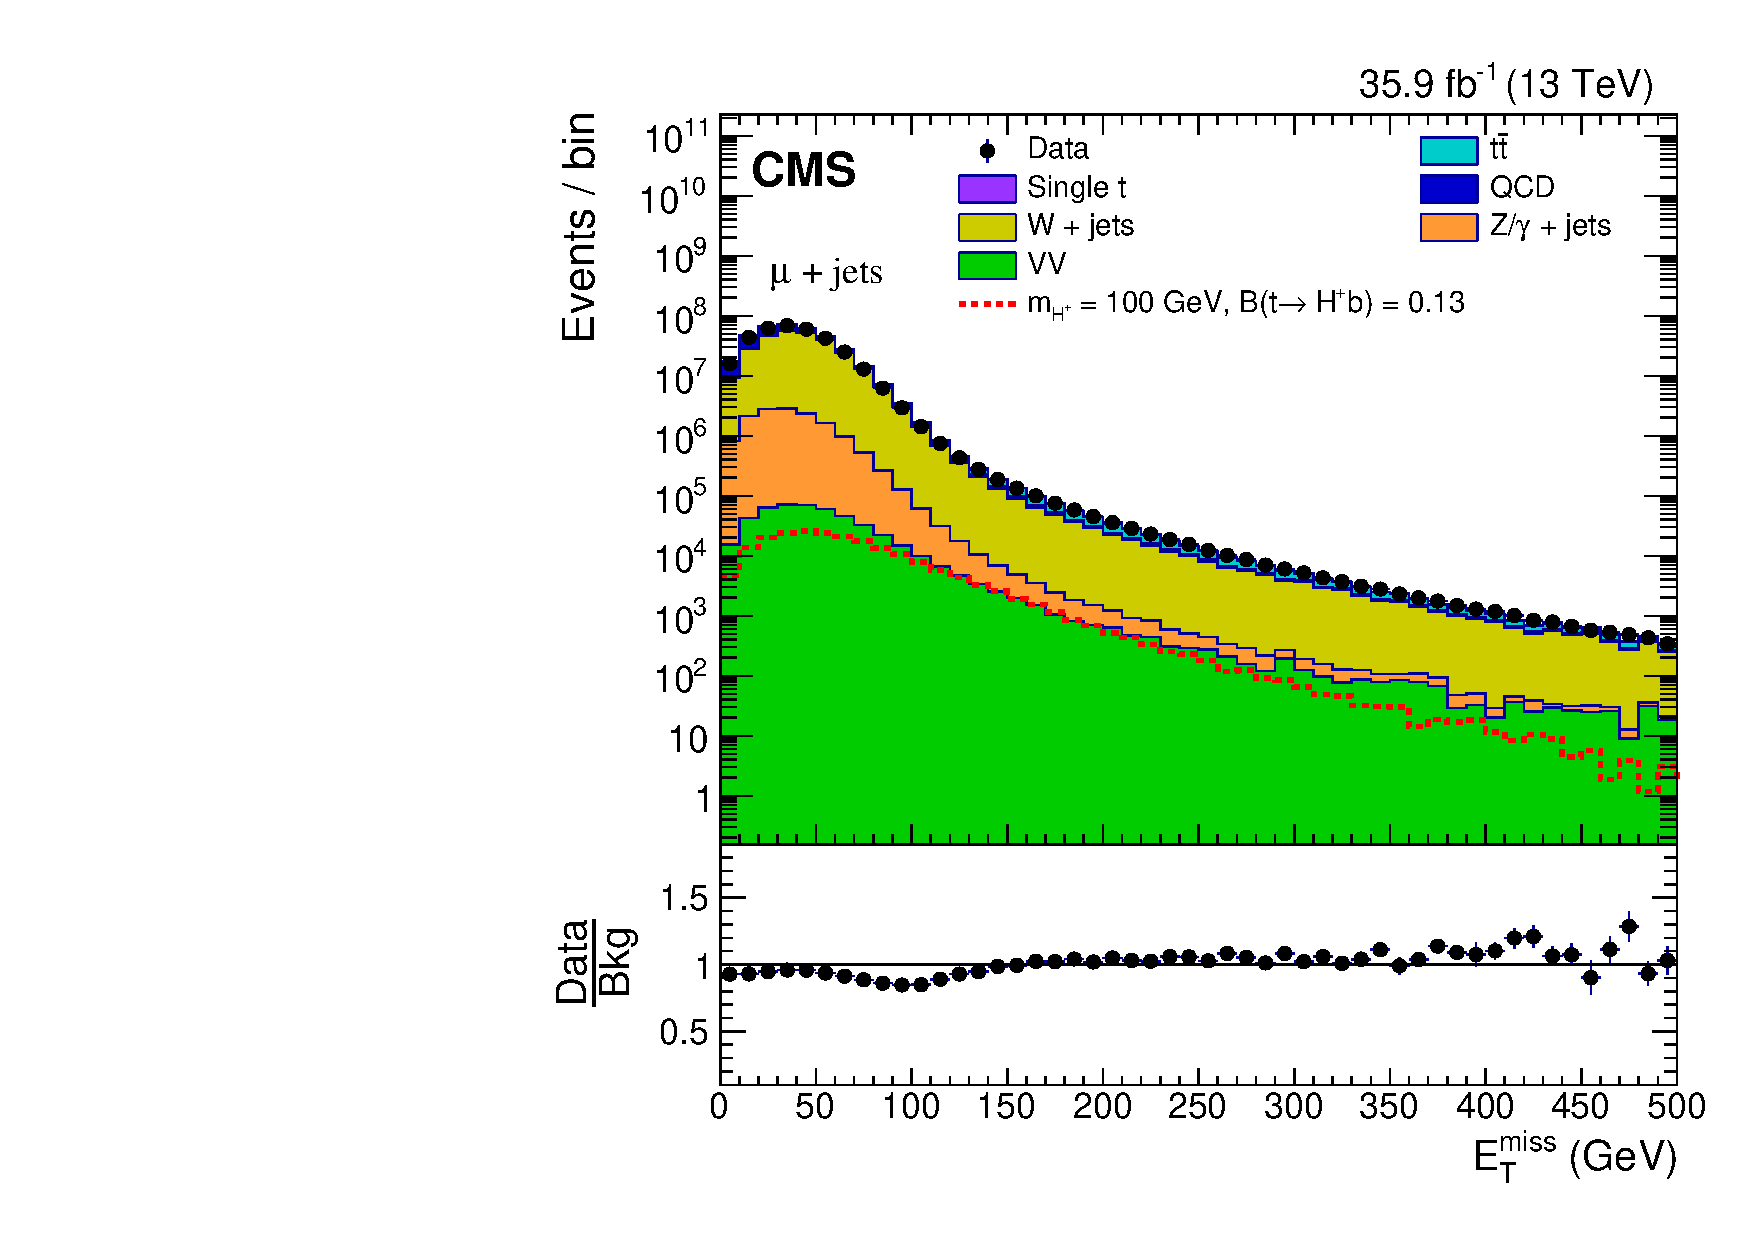
\includegraphics[width=0.49\linewidth]{Image/Muon/pt_met_1Mu_mu.pdf}}
    \subfigure[\label{subfig:pt_met_ele}]
    {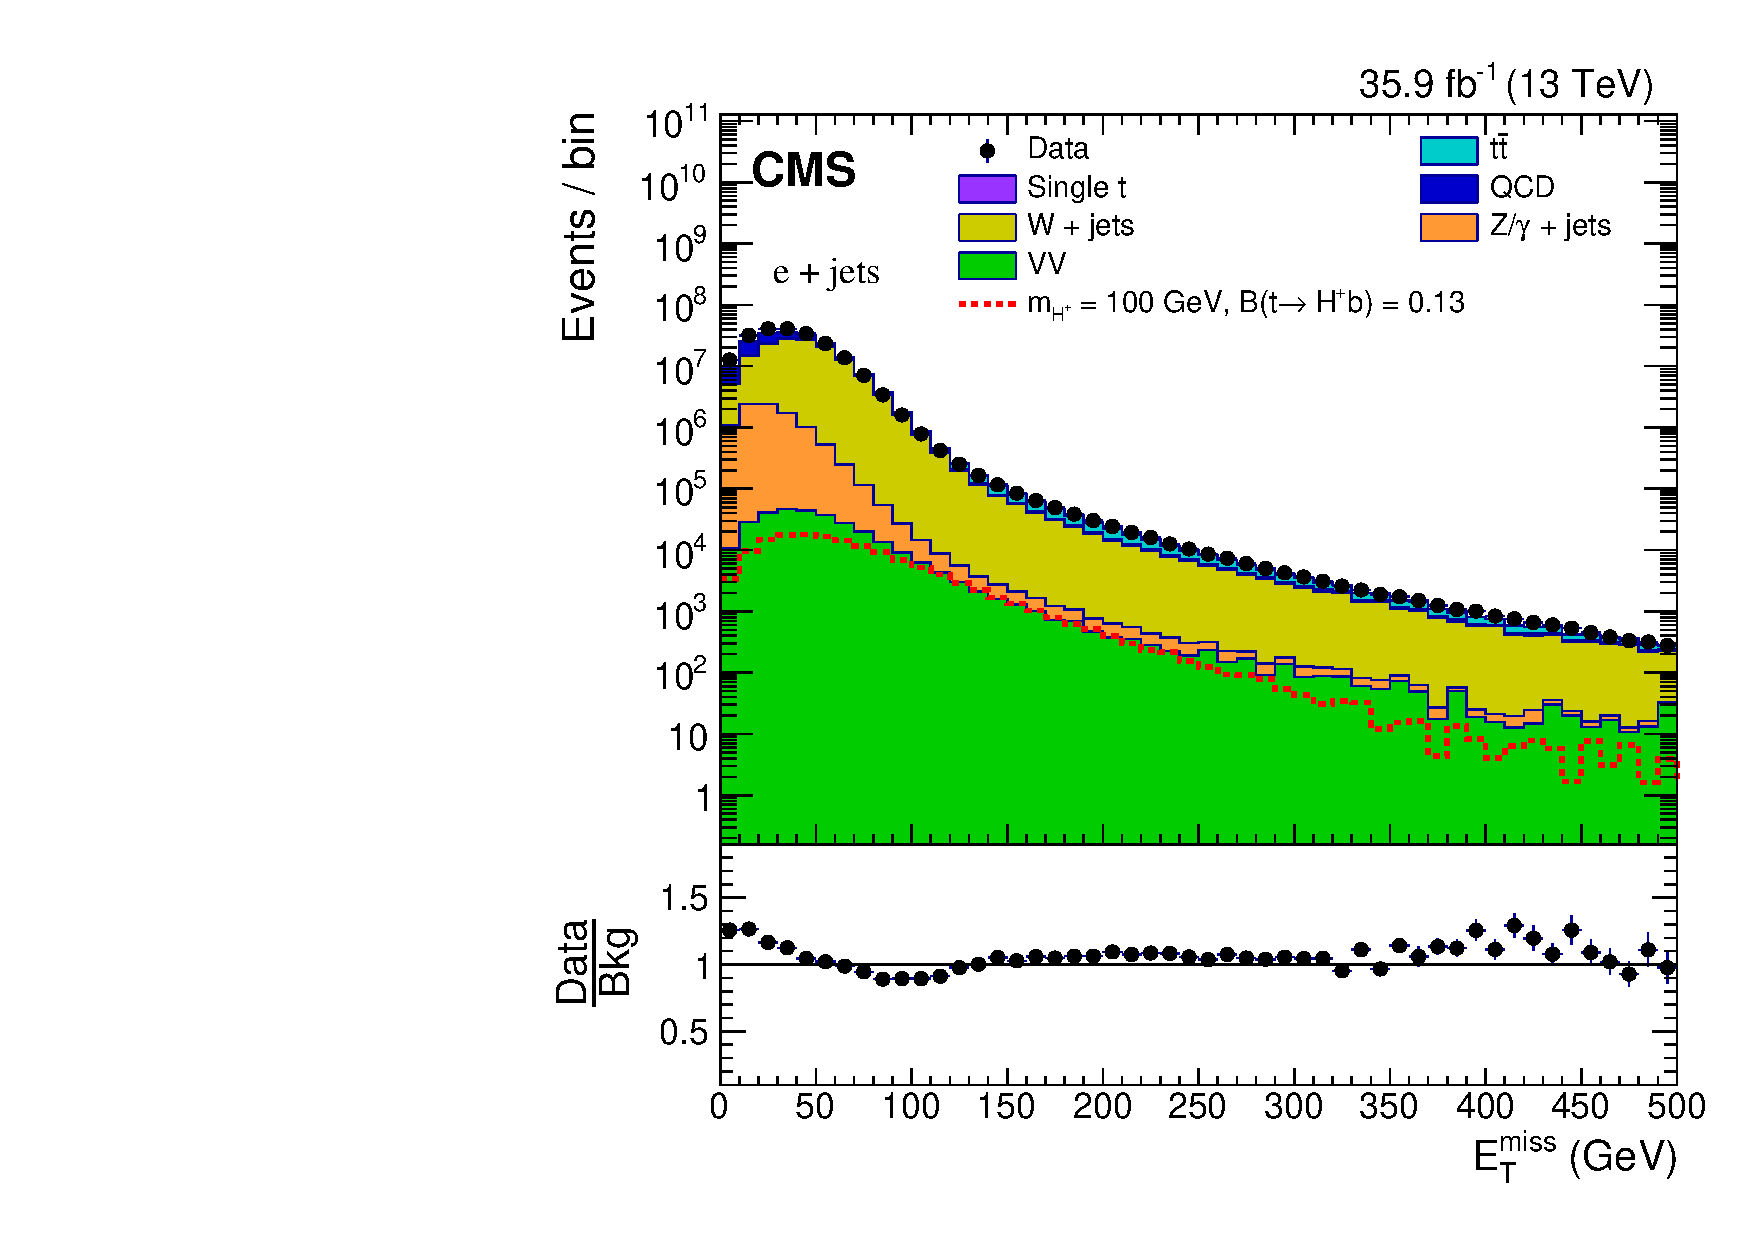
\includegraphics[width=0.49\linewidth]{Image/Electron/pt_met_1Ele_ele.pdf}}
    \caption{Distribution of relative isolation and missing transverse energy after lepton trigger 
	selection for \mujets and \ejets channel. The QCD multijet process is dominated in the high 
	$I_{\text{rel}}$ region.}
    \label{fig:qcdVar}
\end{figure}

\begin{figure}
    \centering  
    \subfigure[\label{subfig:RelIso_MET_TProf_muData}]
    {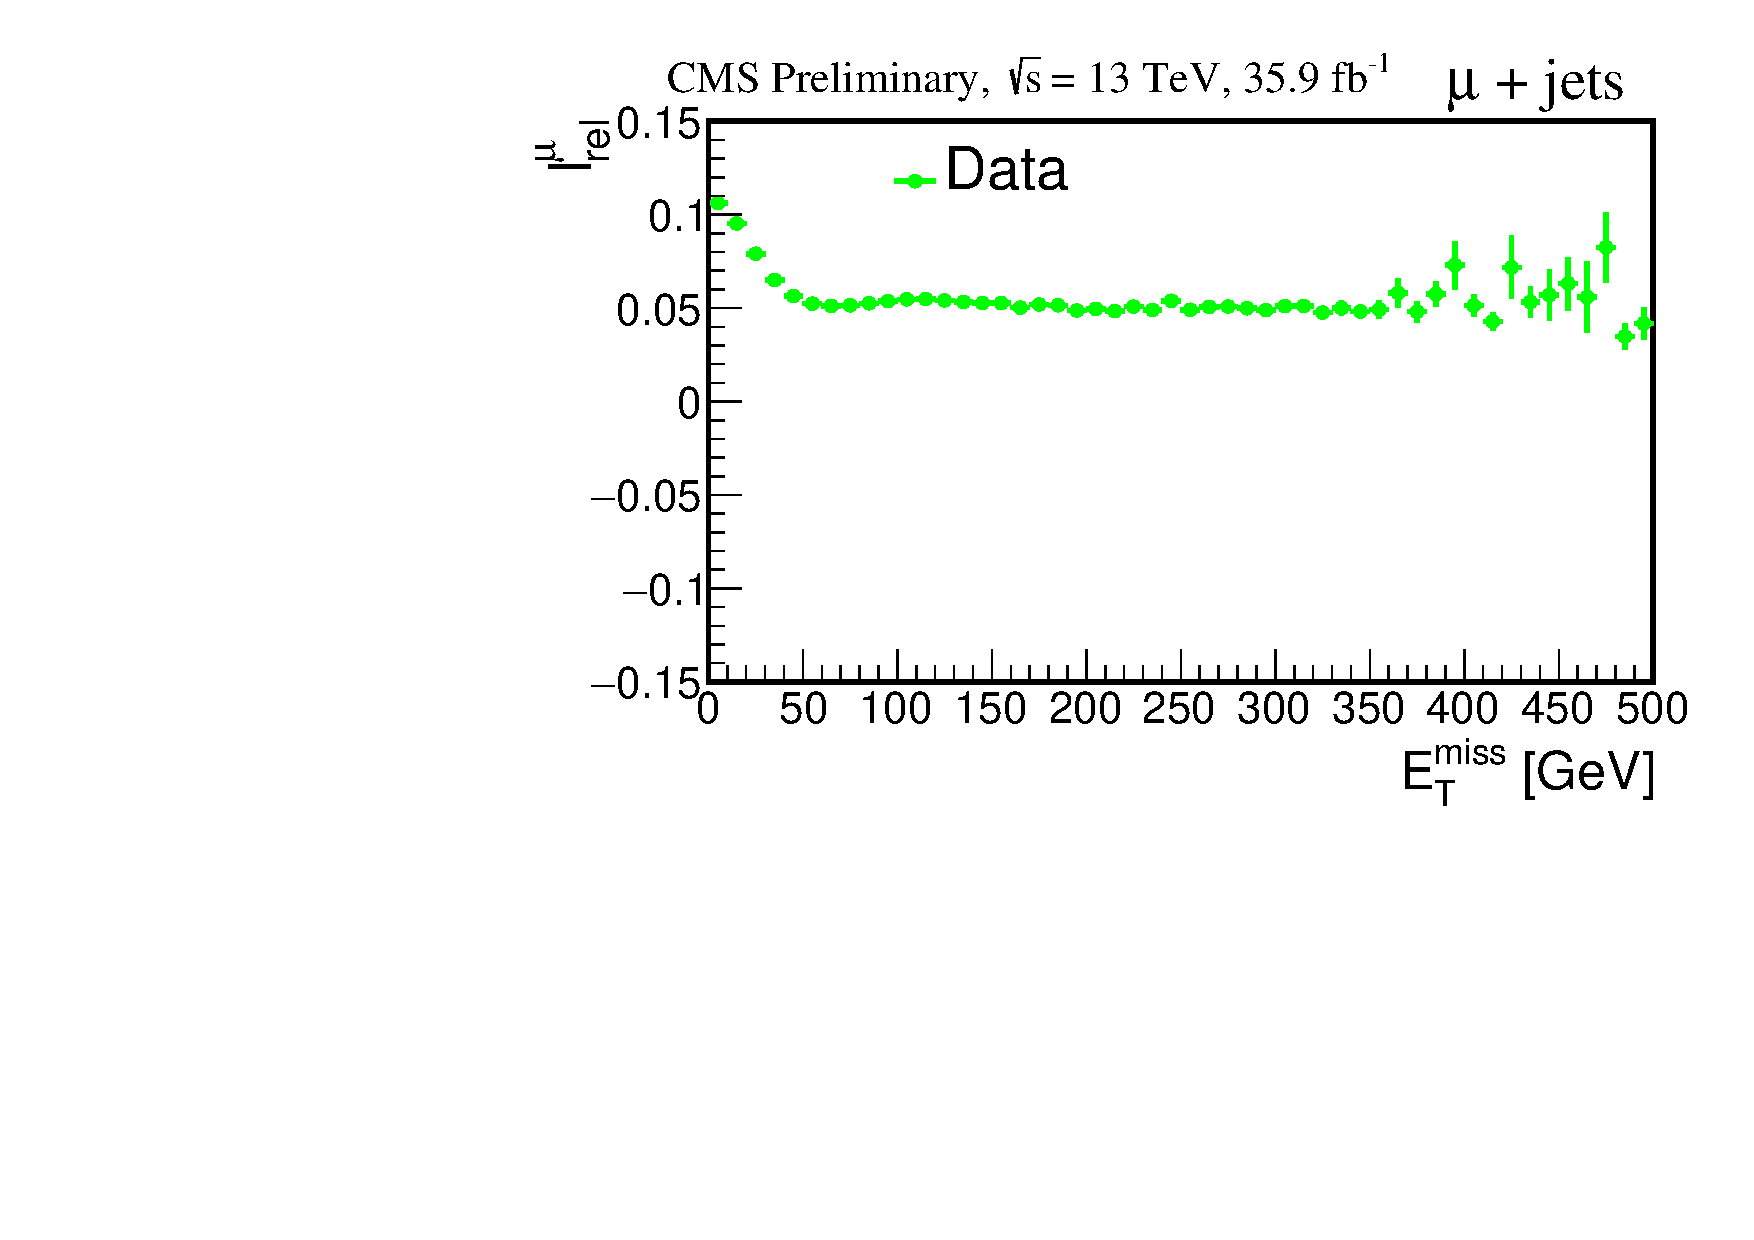
\includegraphics[width=0.49\linewidth]{Image/Muon/RelIso_MET_TProf_muData.pdf}}
    \subfigure[\label{subfig:RelIso_MET_TProf_eleData}]
    {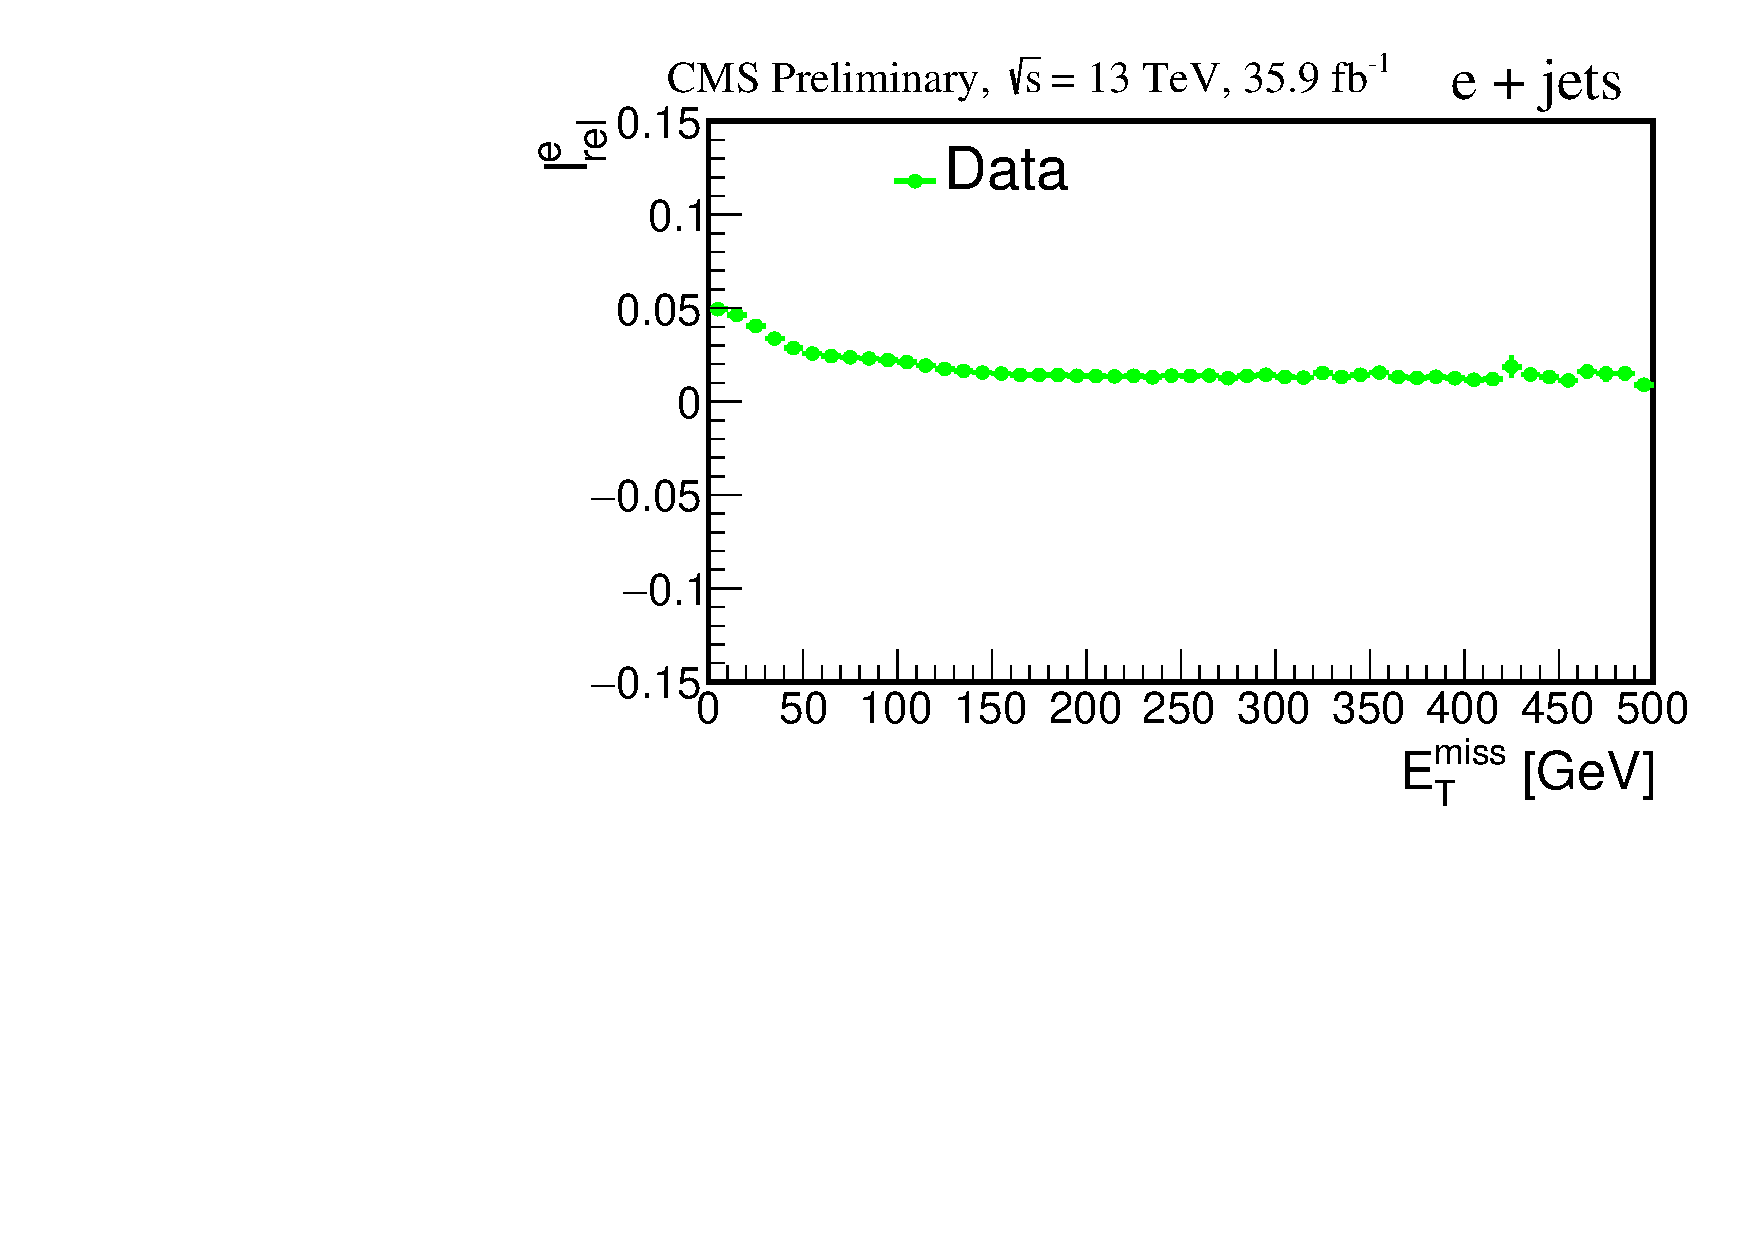
\includegraphics[width=0.49\linewidth]{Image/Electron/RelIso_MET_TProf_eleData.pdf}}
    \vfil
    \subfigure[\label{subfig:RelIso_MET_TProf_muQCD}]
    {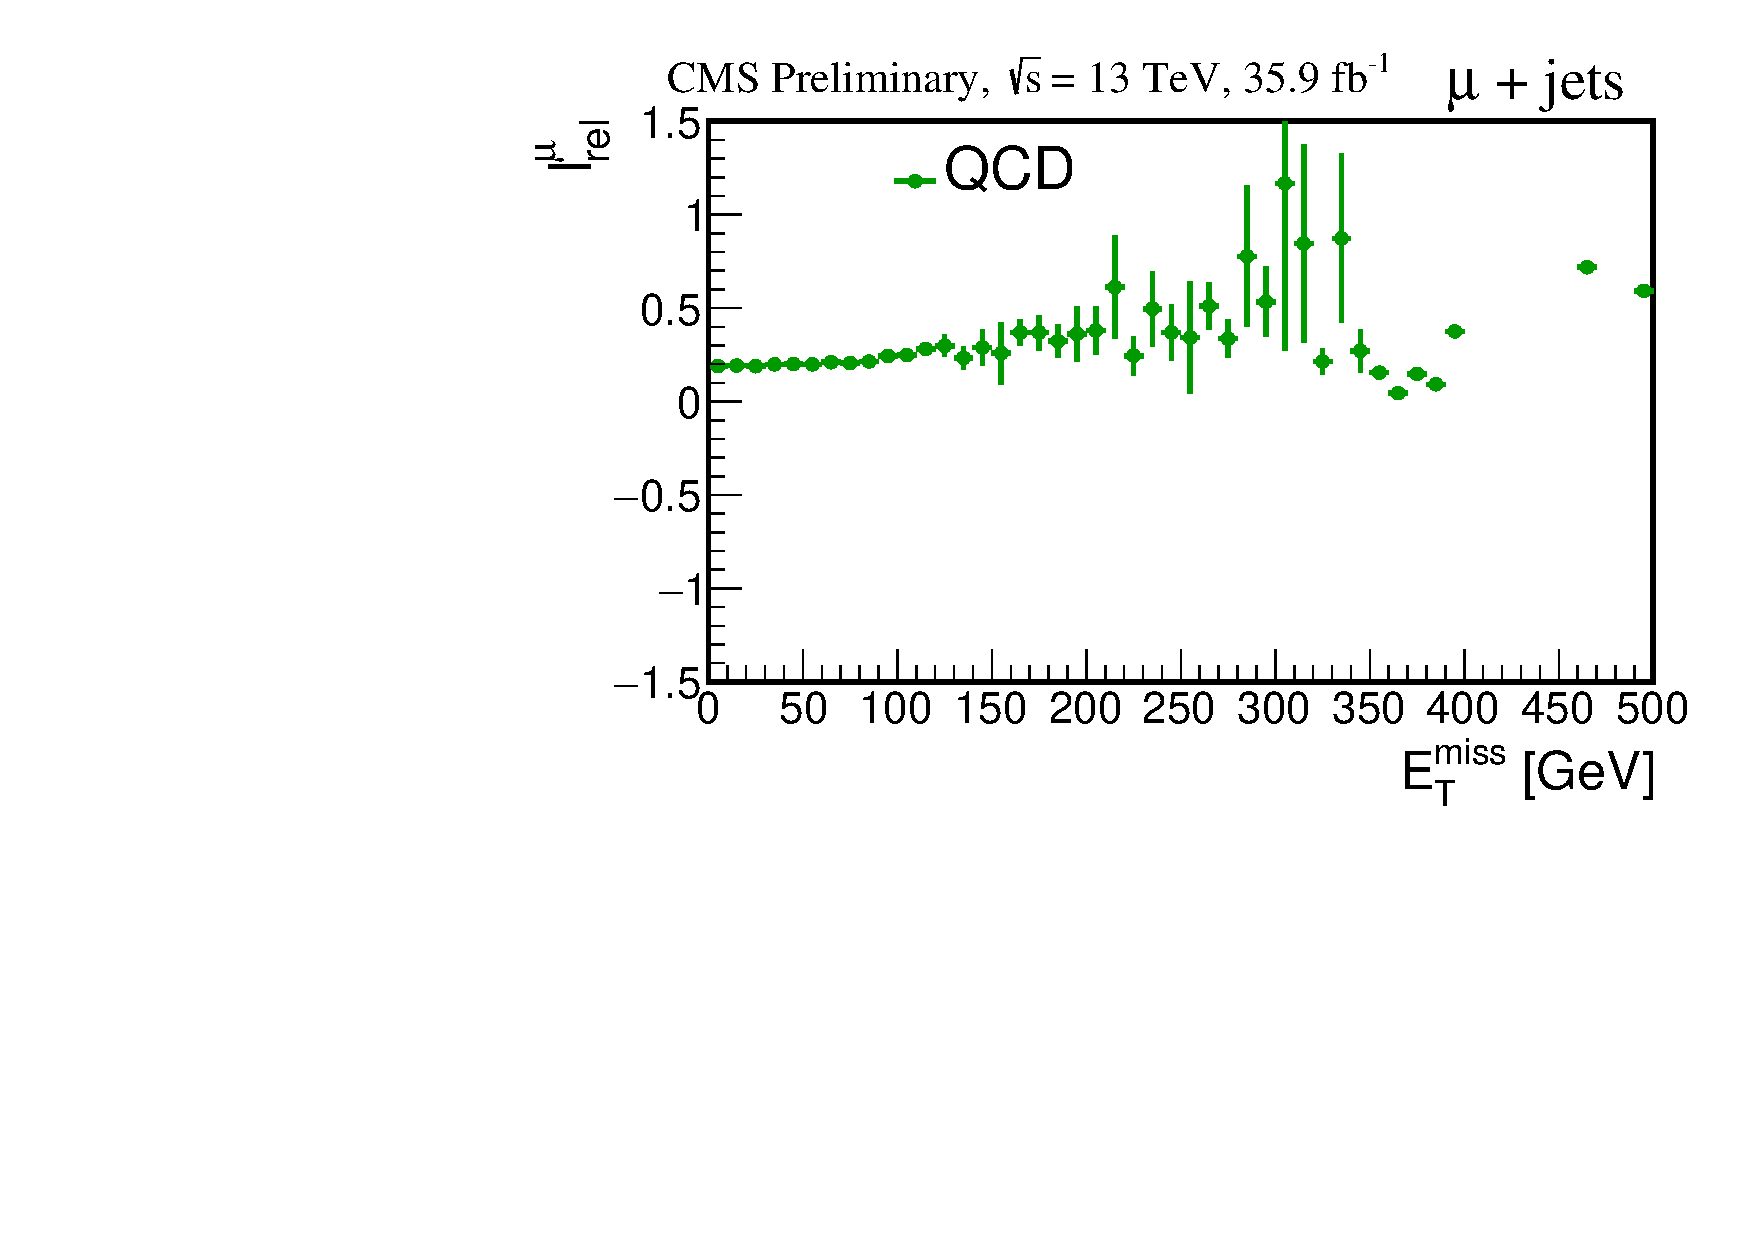
\includegraphics[width=0.49\linewidth]{Image/Muon/RelIso_MET_TProf_muQCD.pdf}}
    \subfigure[\label{subfig:RelIso_MET_TProf_eleQCD}]
    {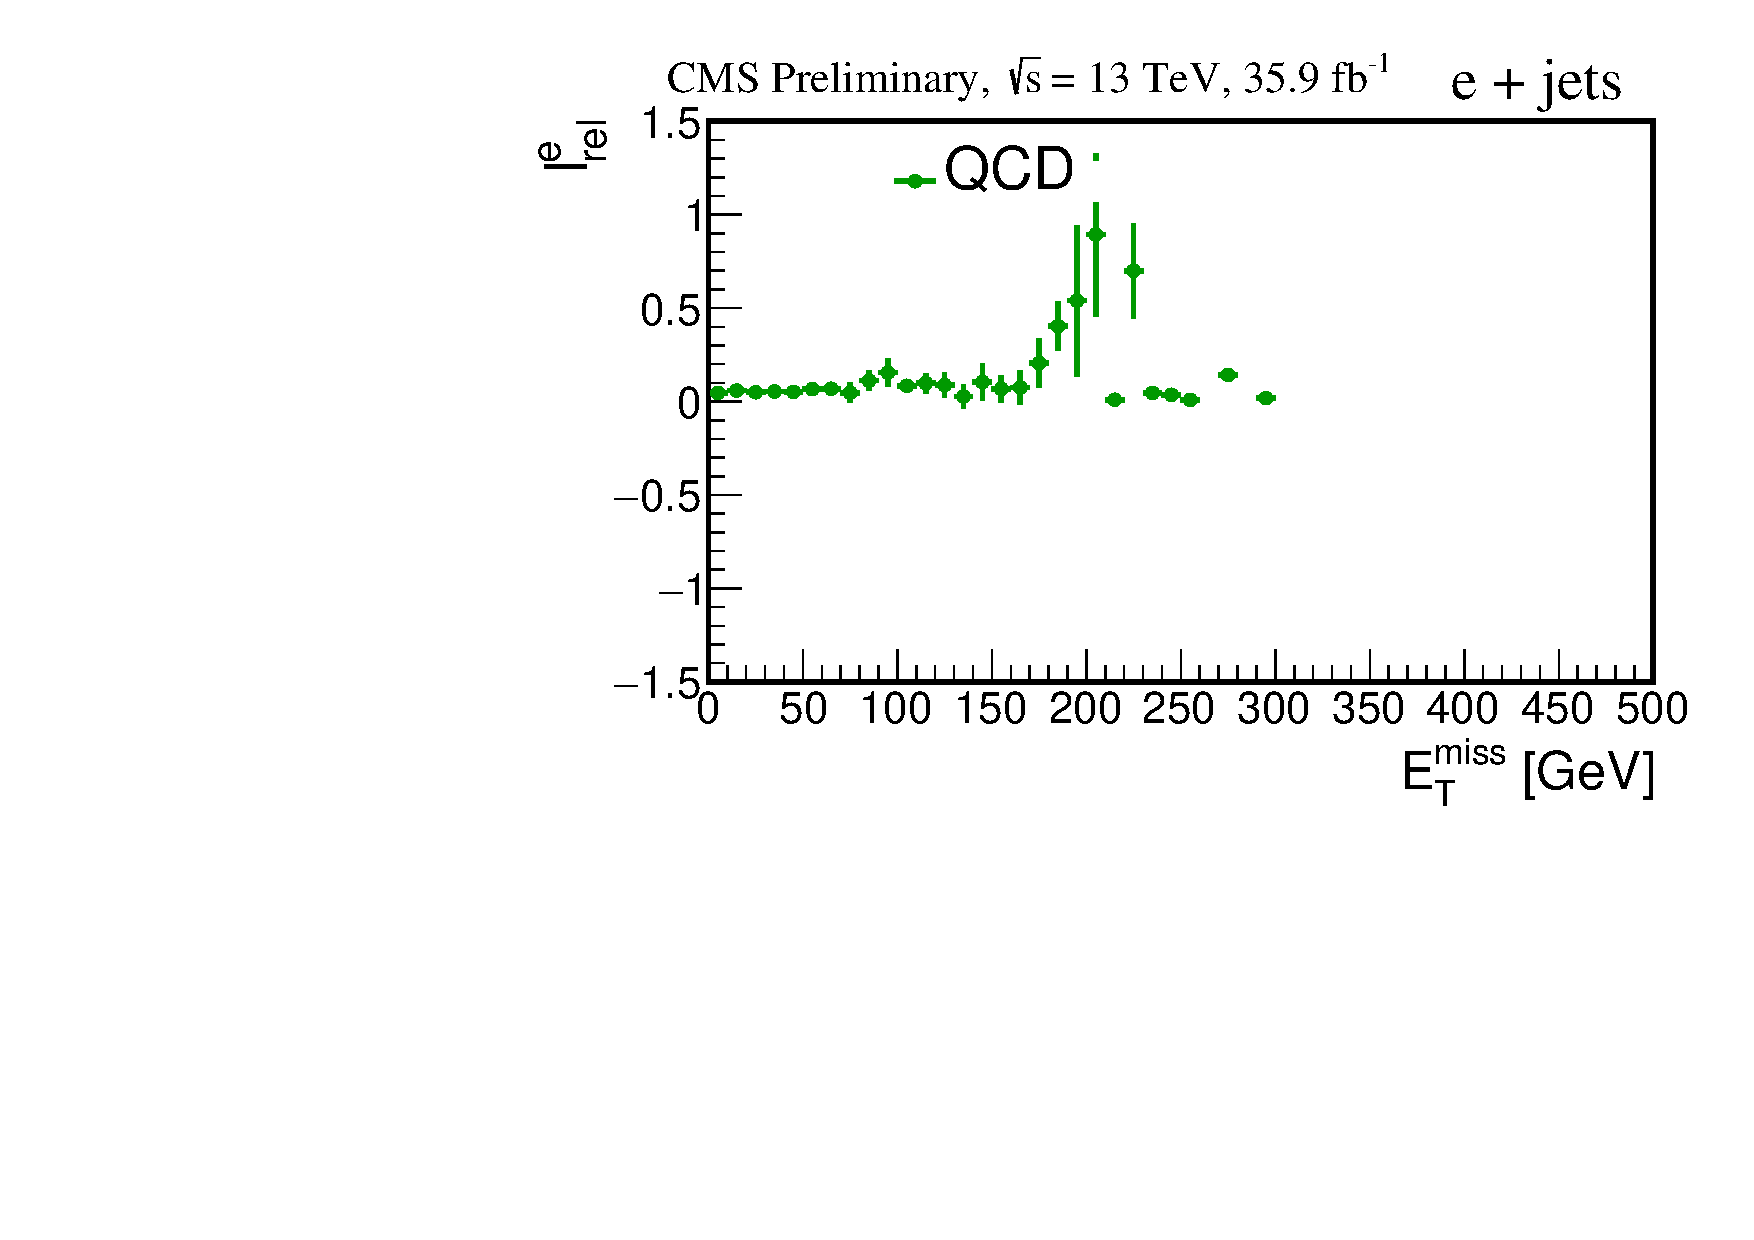
\includegraphics[width=0.49\linewidth]{Image/Electron/RelIso_MET_TProf_eleQCD.pdf}}
    \caption{Distribution of mean of $I_{\text{rel}}$ in different \MET bins after lepton trigger 
	selection for \mujets and \ejets channel. There seems to be some correlation between \MET 
	and $I_{\text{rel}}$ in the low 
	\MET $<$ 50 \GeV region for data as shown in Figures~\ref{subfig:RelIso_MET_TProf_muData},
	\ref{subfig:RelIso_MET_TProf_eleData}. However, from simulated QCD multijet events, 
	the \MET and $I_{\text{rel}}$ are uncorrelated, as shown in 
	Figures~\ref{subfig:RelIso_MET_TProf_muQCD}, \ref{subfig:RelIso_MET_TProf_eleQCD}.}
    \label{fig:qcdVar2}
\end{figure}

\begin{figure}
\begin{center}
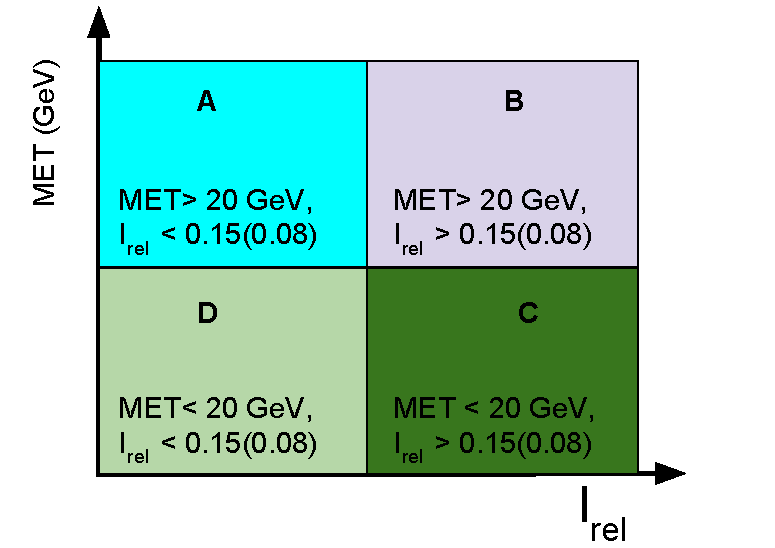
\includegraphics[width=0.70\textwidth]{Image/abcd_region.pdf}
\caption{Different regions between $I_{\text{rel}}$ and MET (missing transverse energy also known as
	\MET) to estimate QCD multijet events from data. For \mujets channel, the isolation region 
	corresponds to $I_{\text{rel}}^{\mu} < 0.15$ whereas the non-isolation corresponds to 
    $0.15 < I_{\text{rel}}^{\mu} < 0.40$. For \ejets channel, the isolation region 
    corresponds to $I_{\text{rel}}^{e} < 0.0821 (0.0695)$ whereas the non-isolation 
    region corresponds to $0.0821 <I_{\text{rel}}^{e} < 0.30$ 
    ($0.0695 <I_{\text{rel}}^{e} < 0.30$) for electron found in barrel (endcap) regions.
}
\label{fig:abcd}
\end{center}
\end{figure}


\subsection{Determination of transfer scale factor}
The phase space of \MET and $I_{\text{rel}}$ are divided into 4 
regions as shown in Figure~\ref{fig:abcd}. The transfer scale factors 
are determined using the following formula 
\begin{equation}
    {\text{SF}_{\text{qcd}}} = \frac{N_{\text{(Data - other backgrounds)}}^\text{D}}{N_{\text {(Data - other backgrounds)}}^\text{C}}
\label{eq:qcdSF}
\end{equation}
The number of events in different regions after kinematic fit 
selection are shown in Table~\ref{tab:qcdABCD_mu} for \mujets and in 
Table~\ref{tab:qcdABCD_ele} for \ejets channel. The 
$\text{SF}_{\text{qcd}}$ is calculated after each selection step, of 
Section~\ref{s:secEvtSel}, using Equation (\ref{eq:qcdSF}). It is to 
be to noted that in some of the bins of a distribution the number of
events in other background is greater than that from data which makes
the difference negative for that bin. The bin content of these negative
bins is set to zero keeping the uncertainty as it is. Therefore, for 
many negative bins there is a larger uncertainty associated with the
transfer factor. For the different distributions, the number of negative
bins is also different which leads to different transfer factor for
them. In this analysis, we compute the transfer factor separately for
each distribution, each channel, and each selection step. The transfer 
scale factors using \mjj distributions after kinematic fit
and charm tagging are shown in Table~\ref{tab:qcdSF} for both 
channels. It can be seen that the transfer scale factors are of 
different orders for the different selection steps.

\begin{table}
\caption{Event yields from different regions, for \mujets channel after kinematic fit selection.}
\label{tab:qcdABCD_mu}
\centering
\begin{adjustbox}{max width=\textwidth}
\begin{tabular}{ccccc}
\hline 
\hline 
\bf{Process} & Region-A & Region-B & Region-C & Region-D  \\ 
 & (Iso, high MET) & (Non iso, high MET) & (Non iso, low MET)& (Iso, low MET) \\ 
\hline 
\hline 
Simulated QCD & 3159 $\pm$ 1022 & 2225$\pm$597 & 1145$\pm$793 & 3221$\pm$2138 \\ 
\hline 
$t\bar{t}$ + jets & 205677 $\pm$ 278 & 10006$\pm$61 & 1006$\pm$20 & 24890$\pm$97 \\ 
Single ~t & 5739 $\pm$ 30 & 262$\pm$7 & 25$\pm$2 & 744$\pm$11 \\ 
 W + jets & 2979 $\pm$ 86 & 149$\pm$19 & 7$\pm$4 & 485$\pm$35 \\ 
$Z/\gamma$ + jets & 441 $\pm$ 17 & 16$\pm$3 & 4$\pm$1 & 120$\pm$8 \\ 
VV & 156 $\pm$ 21 & 6$\pm$5 & 0$\pm$28 & 32$\pm$10 \\ 
\hline 
nonQCDBkg & 216096 $\pm$ 316 & 10440$\pm$65 & 1041$\pm$20 & 26270$\pm$104 \\ 
\hline 
Data & 203178 $\pm$ 451 & 12767$\pm$113 & 1948$\pm$44 & 26307$\pm$162 \\ 
\hline 
\end{tabular}
\end{adjustbox}
\end{table}


\begin{table}
\caption{Event yields from different regions, for \ejets channel after kinematic fit selection.}
\label{tab:qcdABCD_ele}
\centering
\begin{adjustbox}{max width=\textwidth}
\begin{tabular}{ccccc}
\hline 
\hline 
\bf{Process} & Region-A & Region-B & Region-C & Region-D  \\ 
 & (Iso, high MET) & (Non iso, high MET) & (Non iso, low MET)& (Iso, low MET) \\ 
\hline 
\hline 
Simulated QCD & 9798 $\pm$ 6596 & 0$\pm$53 & 49$\pm$49 & 688$\pm$353 \\ 
\hline 
$t\bar{t}$ + jets & 143178 $\pm$ 228 & 3931$\pm$38 & 424$\pm$12 & 18398$\pm$82 \\ 
Single ~t & 4030 $\pm$ 25 & 97$\pm$4 & 9$\pm$1 & 544$\pm$9 \\ 
 W + jets & 2115 $\pm$ 72 & 47$\pm$10 & 2$\pm$2 & 344$\pm$28 \\ 
$Z/\gamma$ + jets & 453 $\pm$ 15 & 11$\pm$2 & 4$\pm$1 & 191$\pm$11 \\ 
VV & 67 $\pm$ 13 & 0$\pm$53 & 0$\pm$18 & 31$\pm$8 \\ 
\hline 
nonQCDBkg & 154153 $\pm$ 309 & 4086$\pm$39 & 439$\pm$13 & 19508$\pm$88 \\ 
\hline 
Data & 148499 $\pm$ 385 & 6995$\pm$84 & 1271$\pm$36 & 20740$\pm$144 \\ 
\hline 
\end{tabular}
\end{adjustbox}
\end{table}

\begin{table}
\begin{center}
\begin{tabular}{ccc}
\multicolumn{3}{c}{ } \\
\hline
\hline
\multicolumn{1}{c}{{\bf{Cuts}}} & \multicolumn{1}{c}{$\text{SF}_{\text{qcd}}$} & \multicolumn{1}{c}{$\text{SF}_{\text{qcd}}$}\\
           &( \mujets)  & (\ejets) \\
\hline                                                           
\hline
$N_{\text{\PQb jets}}\geq$2& 1.345 $\pm$ 0.133   & 1.851 $\pm$ 0.117  \\
Kinematic fit selection    & 0.474 $\pm$ 0.214   & 1.481 $\pm$ 0.214  \\
$N_{\text{\PQc jets}}\geq$1& 0.396 $\pm$ 0.217   & 1.395 $\pm$ 0.215  \\
\hline
Exclusive loose     & 0.325 $\pm$ 0.281   & 1.017 $\pm$ 0.267  \\
Exclusive medium    & 0.629 $\pm$ 0.425   & 1.267 $\pm$ 0.412  \\
Exclusive tight     & 0.717 $\pm$ 0.782   & 1.279 $\pm$ 0.742  \\
\hline                                                          
\end{tabular}
\caption{The QCD multijet transfer scale factors ($\text{SF}_{\text{qcd}}$) for \mujets and \ejets 
channel after various selection steps. The categorization of events based on exclusive loose, medium, 
and tight \PQc quark tagging is described in Section~\ref{s:secMjjCat}.}
\label{tab:qcdSF}
\end{center}
\end{table}


\subsection{Estimation of QCD multijet in the signal region}
All the other backgrounds are subtracted from data in region-B and the resulting distribution 
is multiplied with the transfer scale factor to estimate the contribution of data-driven QCD multijet
 events in region-A (signal region) i.e. 
\begin{equation}
    (\text{QCD})_\text{A} = \text{SF}_{\text{qcd}}\times (\text{Data - other backgrounds})_\text{B} 
\end{equation}
In the control plots of Figures~\ref{fig:btagPlot1}, \ref{fig:btagPlot2}, \ref{fig:btagPlot3} and 
\ref{fig:kfitPlot1}, \ref{fig:kfitPlot2}, \ref{fig:kfitPlot3}, the data-driven QCD multijet events are
shown.

\subsection{Comparison of data-driven QCD multijet shapes}
The validity of ABCD method relies on the fact that the data-driven QCD multijet shape should be 
similar in all the four regions. For sake of comparison, we compare shapes of few variables after
\PQb jet and kinematic fit selection steps. In the low \MET region, the shape of \pt, $\eta$ of 
jets and lepton from the isolated and anti-isolated region are shown in 
Figures~\ref{fig:qcd_shape_btag},~\ref{fig:qcd_shape_kinfit}. From these figures, it can be seen that 
the data-driven shape in isolated and anti-isolated matches quite well for these distributions. In few
bins, the number of events in other background is greater than that in data. Therefore the number of
data-driven QCD multijet events ($n_{\text{Data - other background}}$) becomes negative. We set bin 
content of such bin to zero keeping the statistical uncertainty as it is. 
\begin{figure}
    \centering  
    \subfigure[$\eta$ of muon \label{subfig:mu_BTag_eta_mu.pdf}]
    {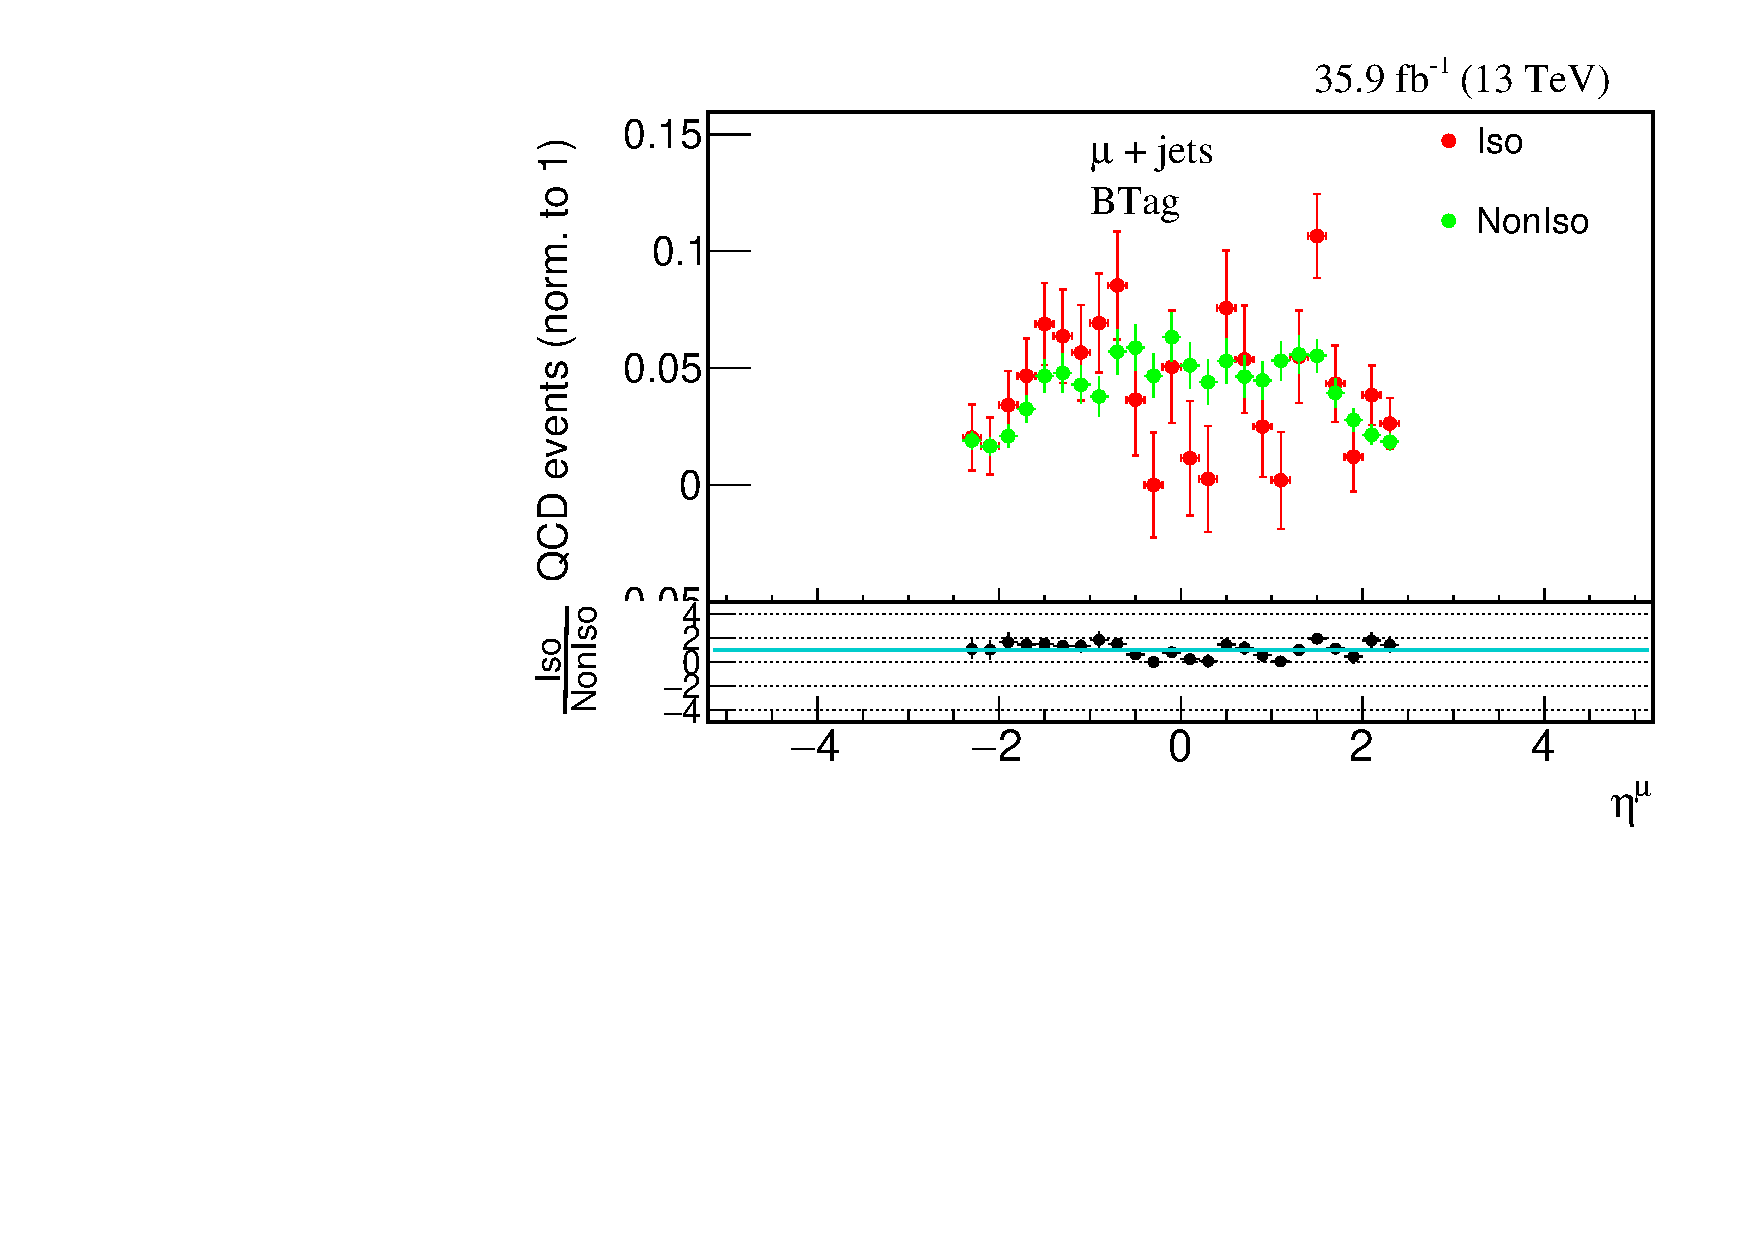
\includegraphics[width=0.40\linewidth]{Image/Muon/QCD/mu_BTag_eta_mu.pdf}}
    \subfigure[$\eta$ of electron \label{subfig:ele_BTag_eta_ele.pdf}]
    {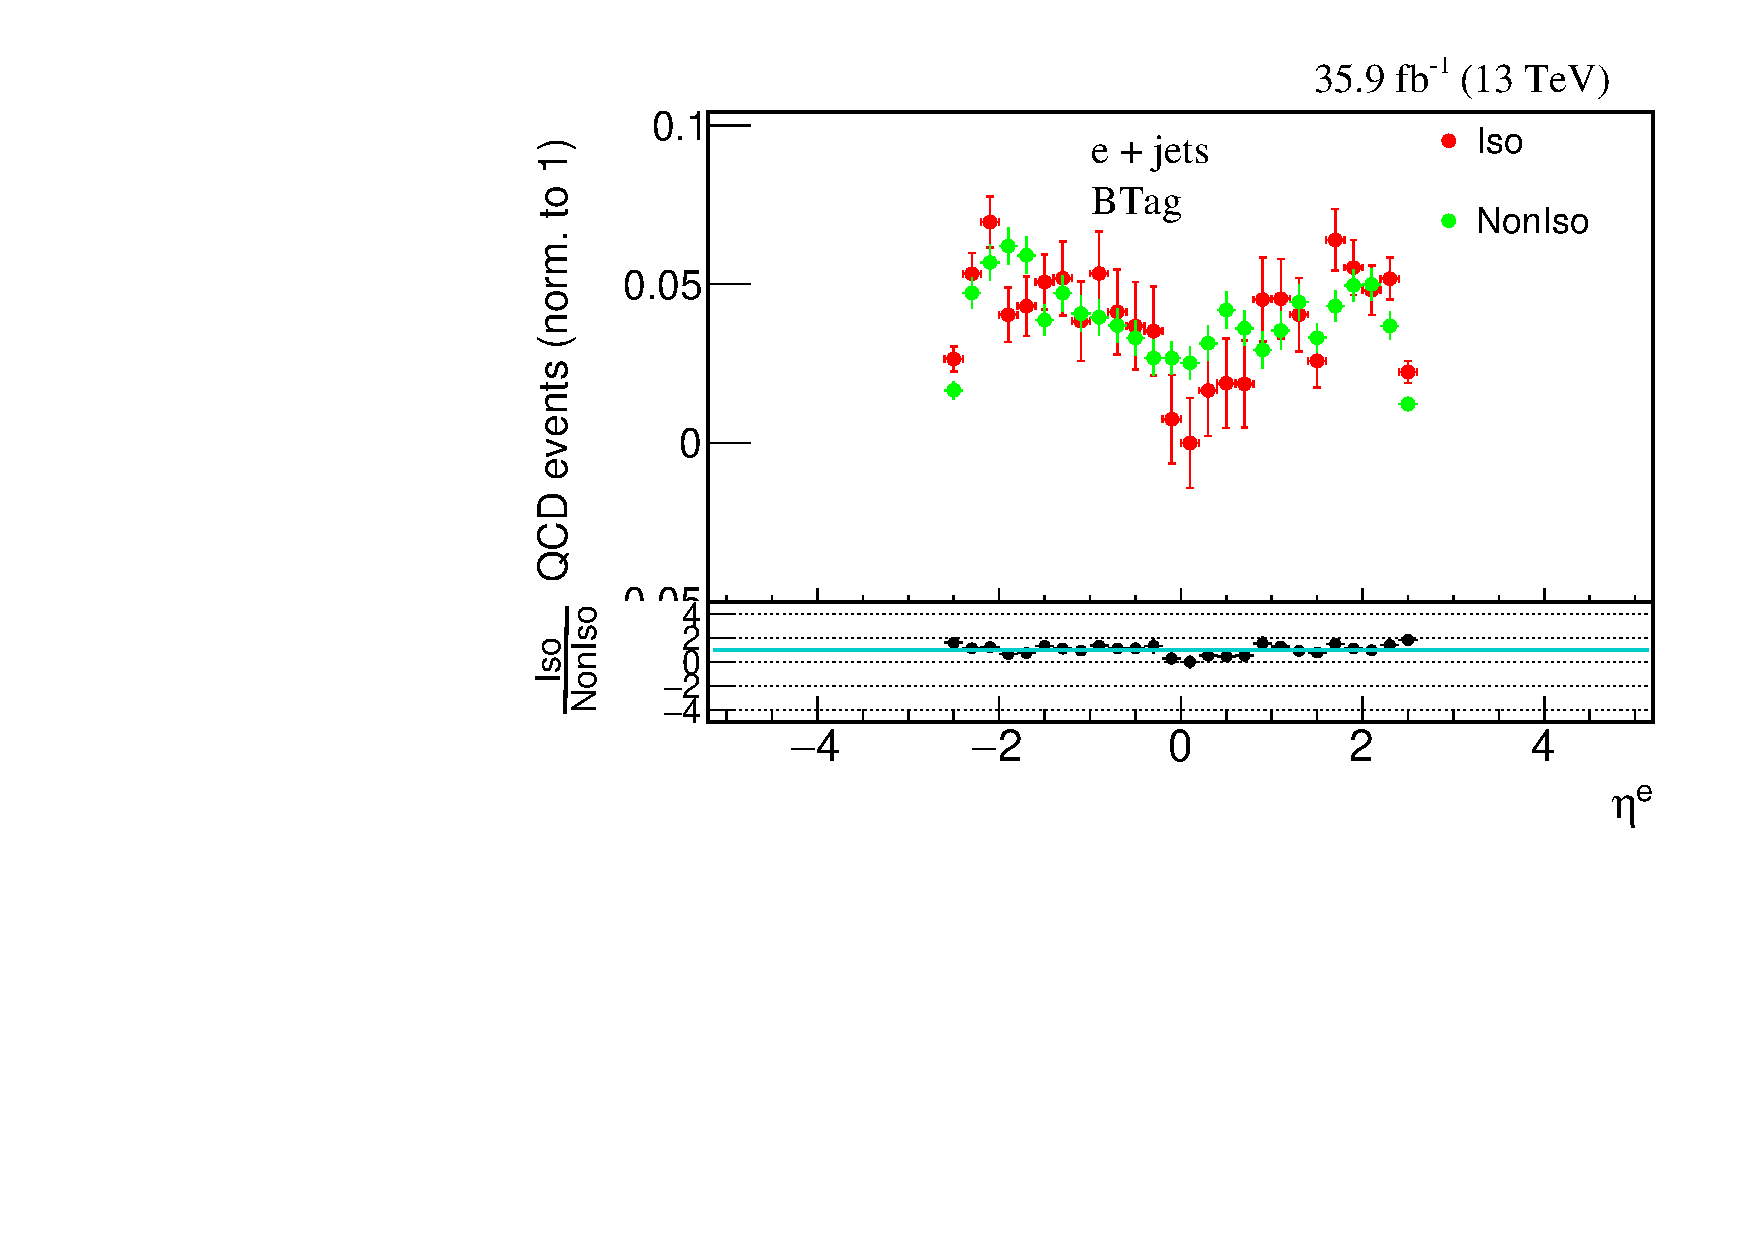
\includegraphics[width=0.40\linewidth]{Image/Electron/QCD/ele_BTag_eta_ele.pdf}}
    \vfil
    \subfigure[$\eta$ of jets \label{subfig:mu_BTag_eta_jet.pdf}]
    {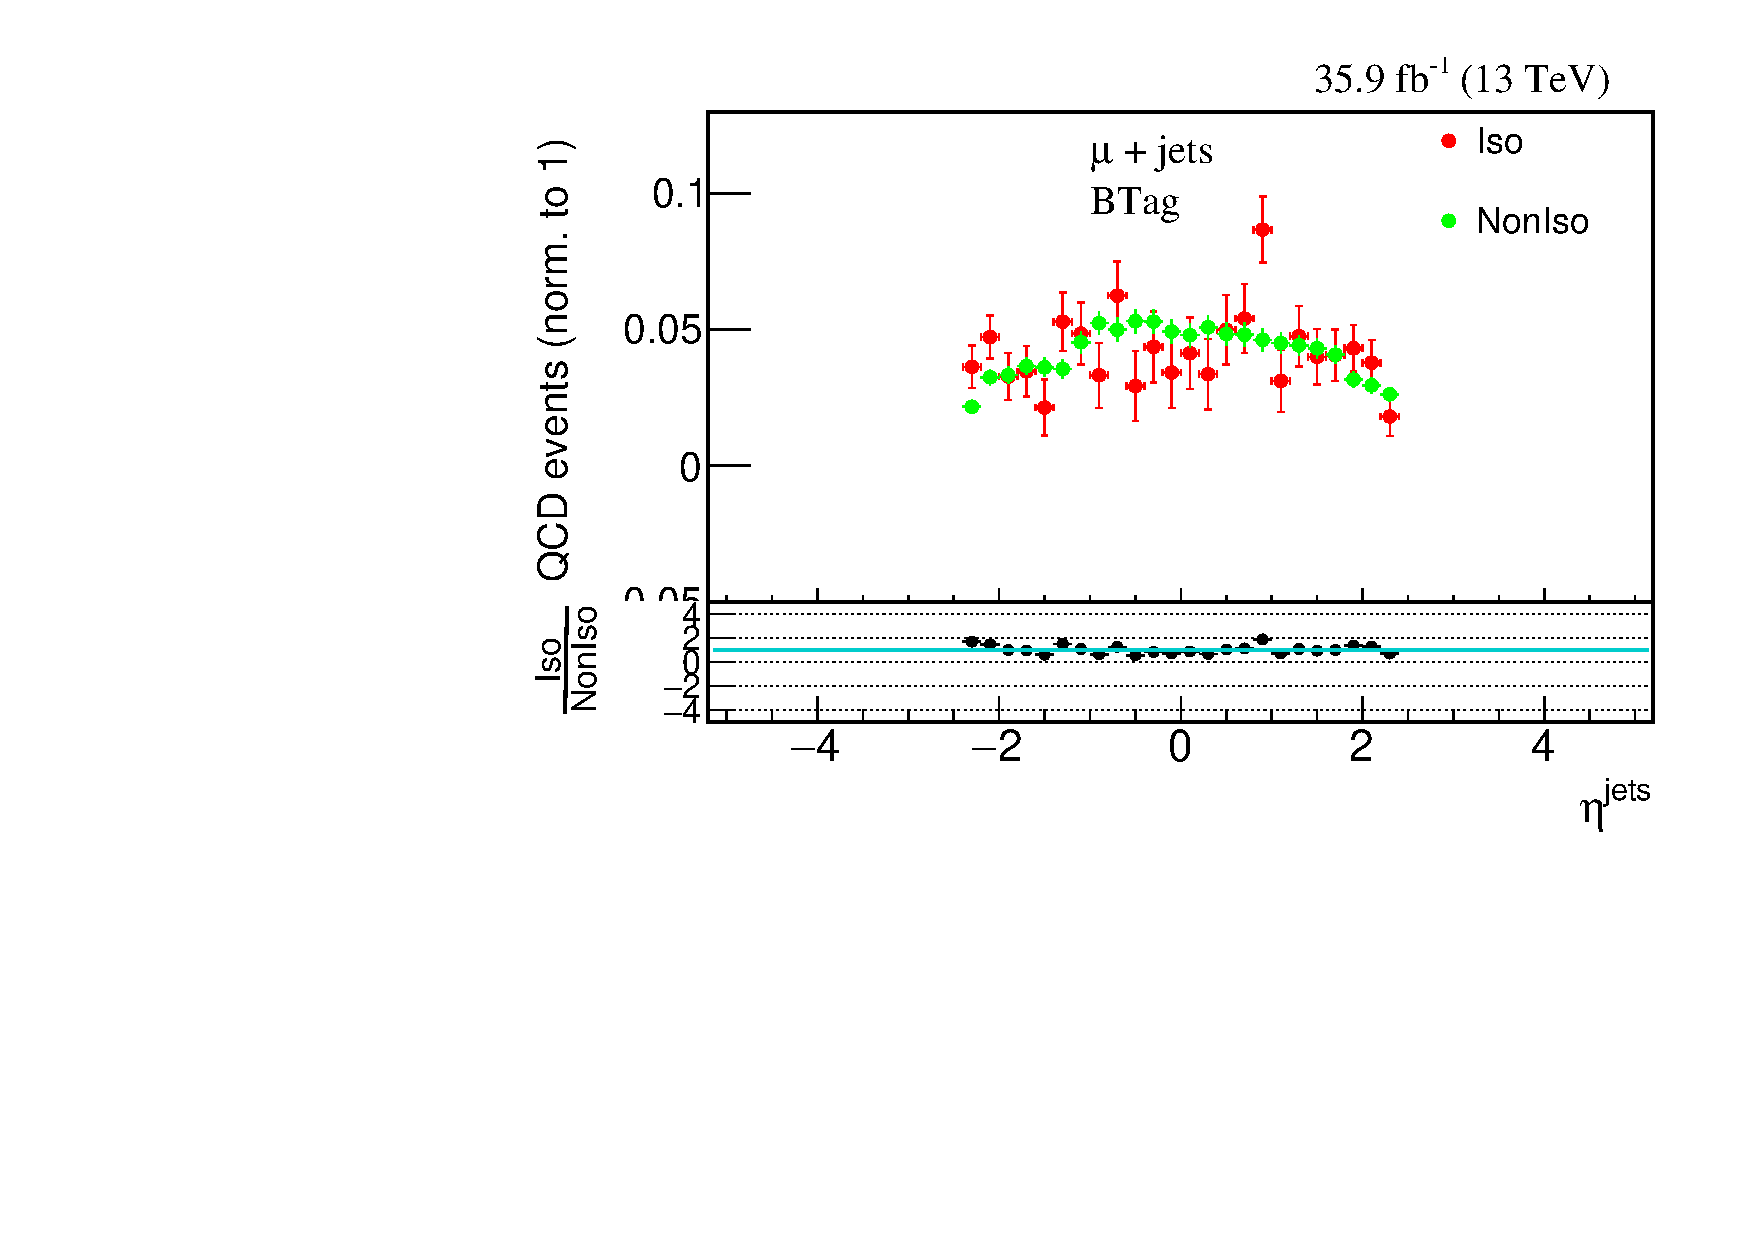
\includegraphics[width=0.40\linewidth]{Image/Muon/QCD/mu_BTag_eta_jet.pdf}}
    \subfigure[$\eta$ of jets \label{subfig:ele_BTag_eta_jet.pdf}]
    {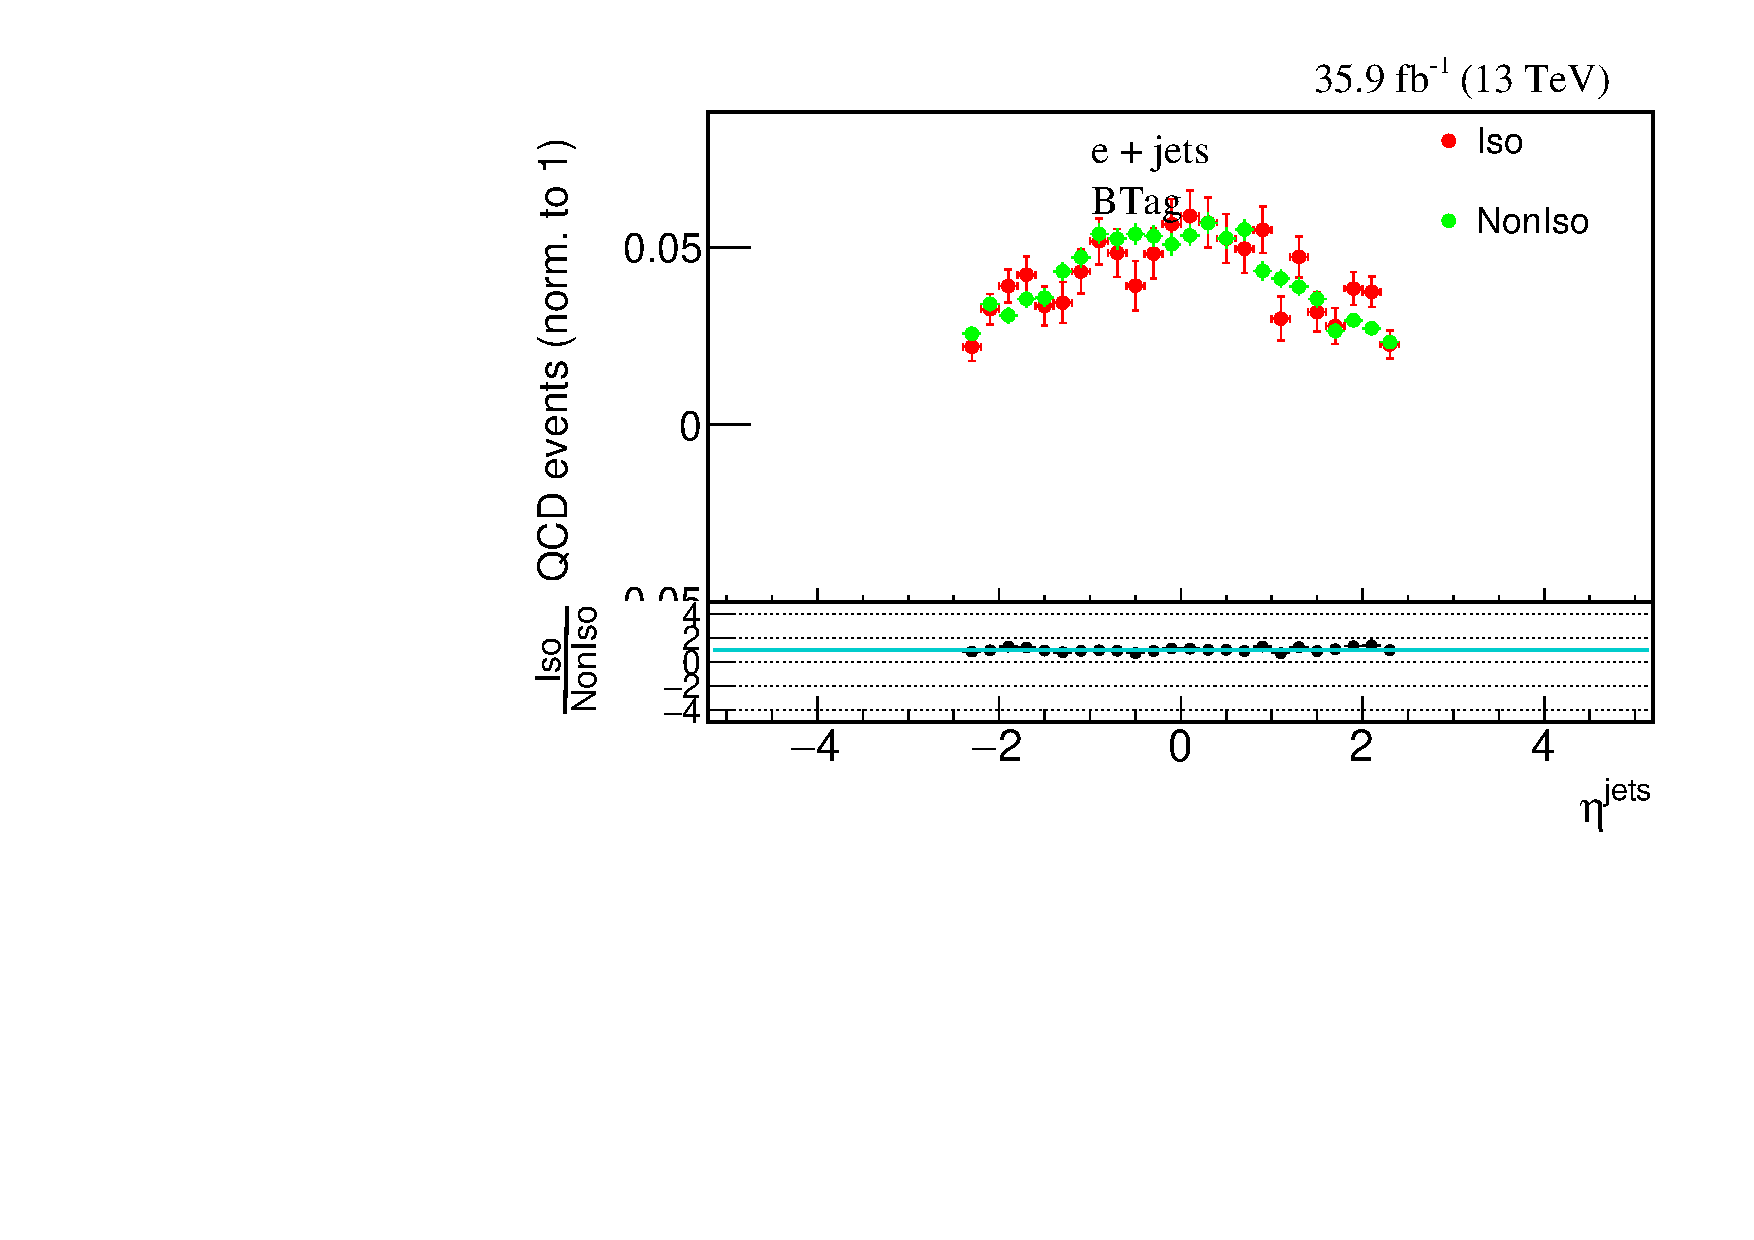
\includegraphics[width=0.40\linewidth]{Image/Electron/QCD/ele_BTag_eta_jet.pdf}}
    \vfil
    \subfigure[$\pt$ of muon \label{subfig:mu_BTag_pt_mu.pdf}]
    {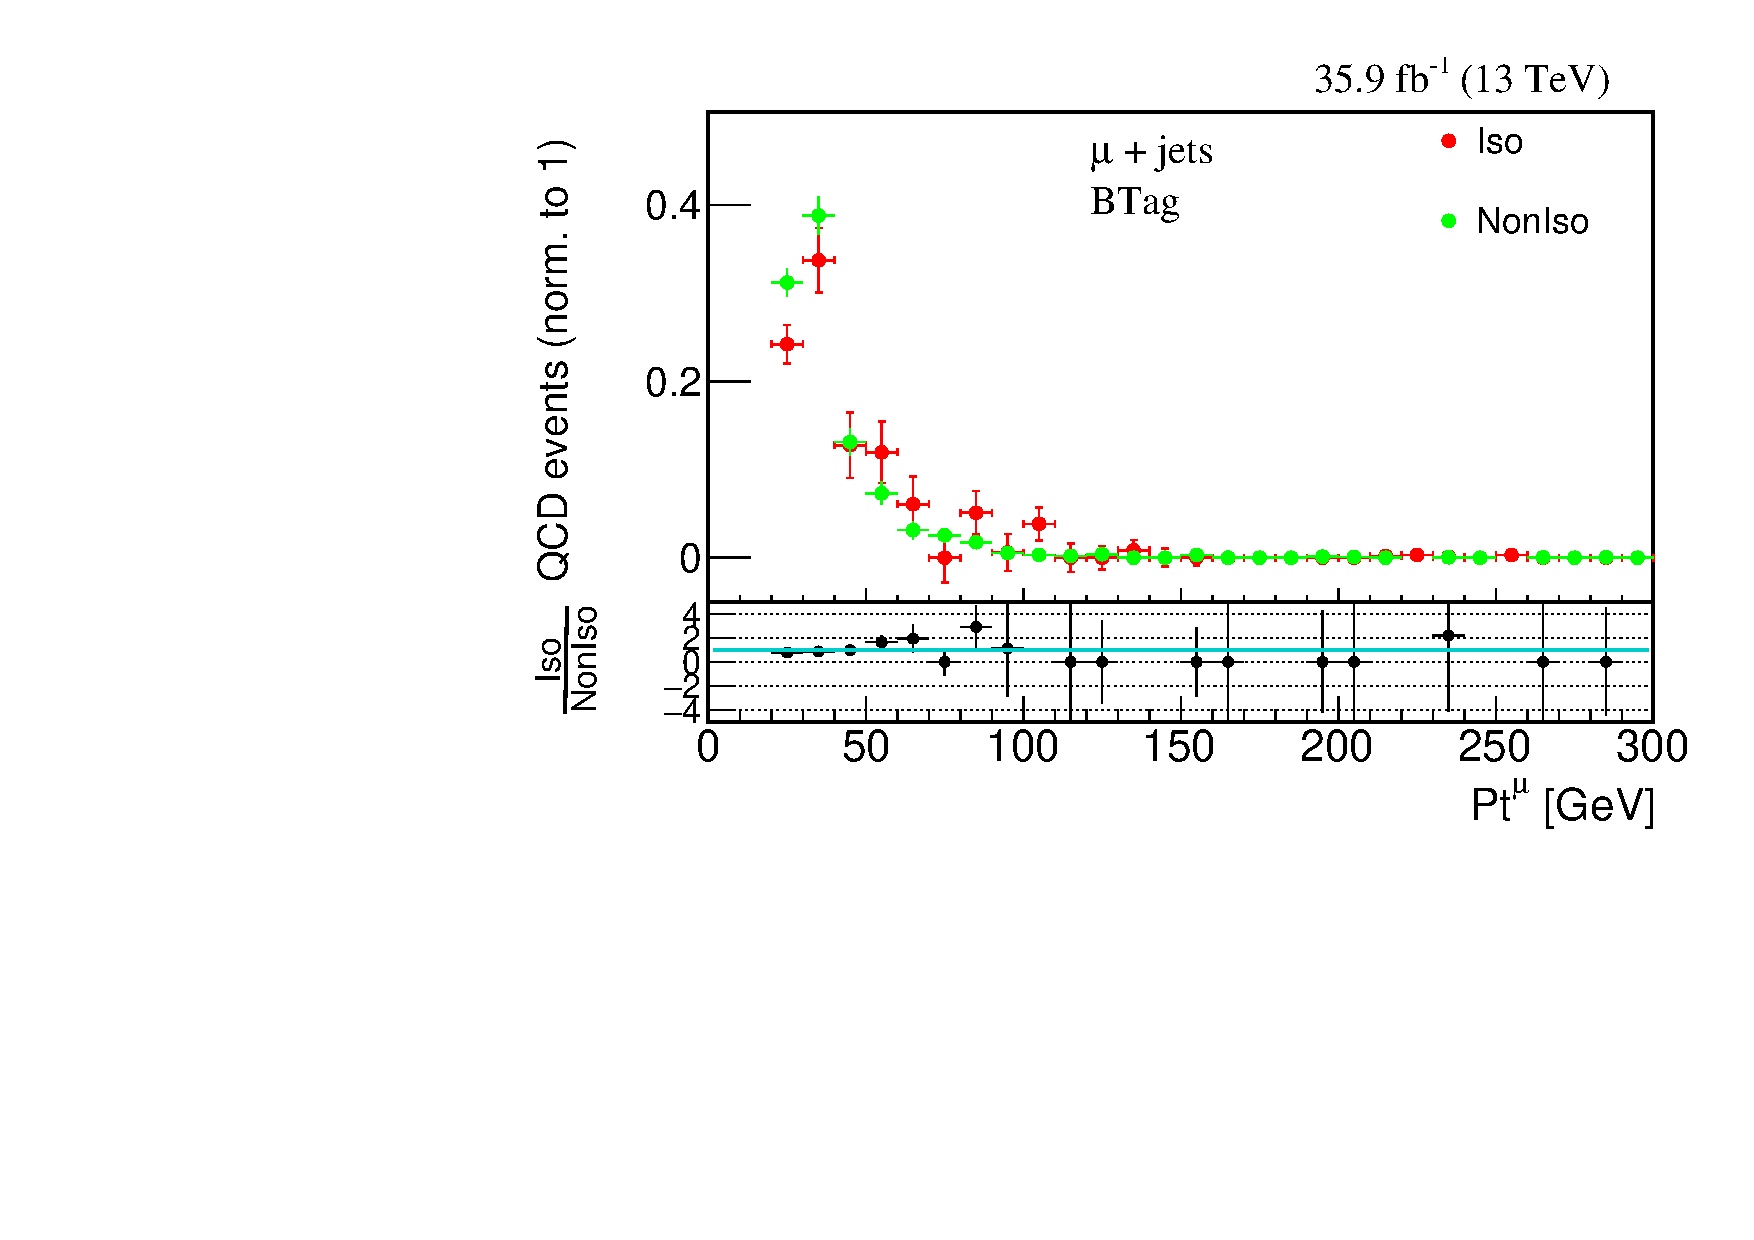
\includegraphics[width=0.40\linewidth]{Image/Muon/QCD/mu_BTag_pt_mu.pdf}}
    \subfigure[$\pt$ of electron \label{subfig:ele_BTag_pt_ele.pdf}]
    {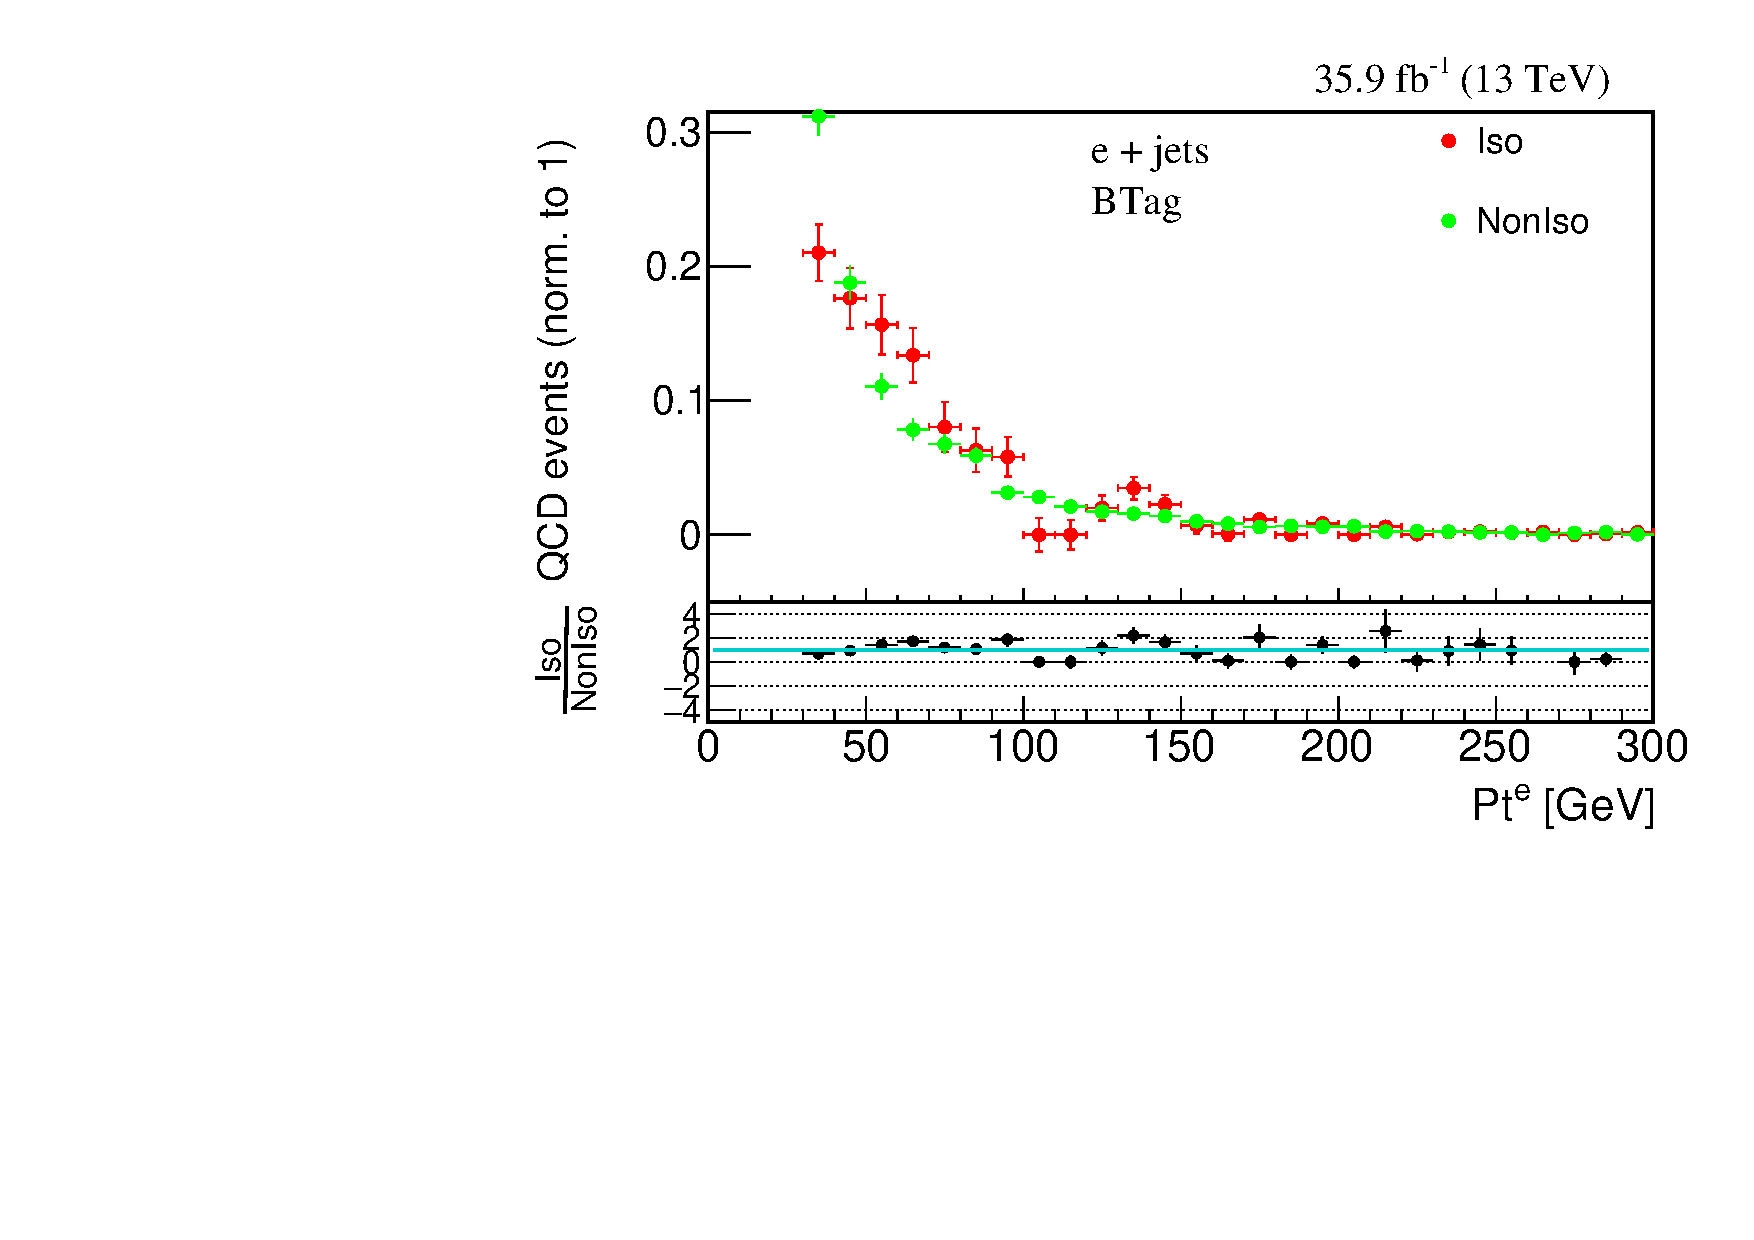
\includegraphics[width=0.40\linewidth]{Image/Electron/QCD/ele_BTag_pt_ele.pdf}}
    \vfil
    \subfigure[$\pt$ of jets \label{subfig:mu_BTag_pt_jet.pdf}]
    {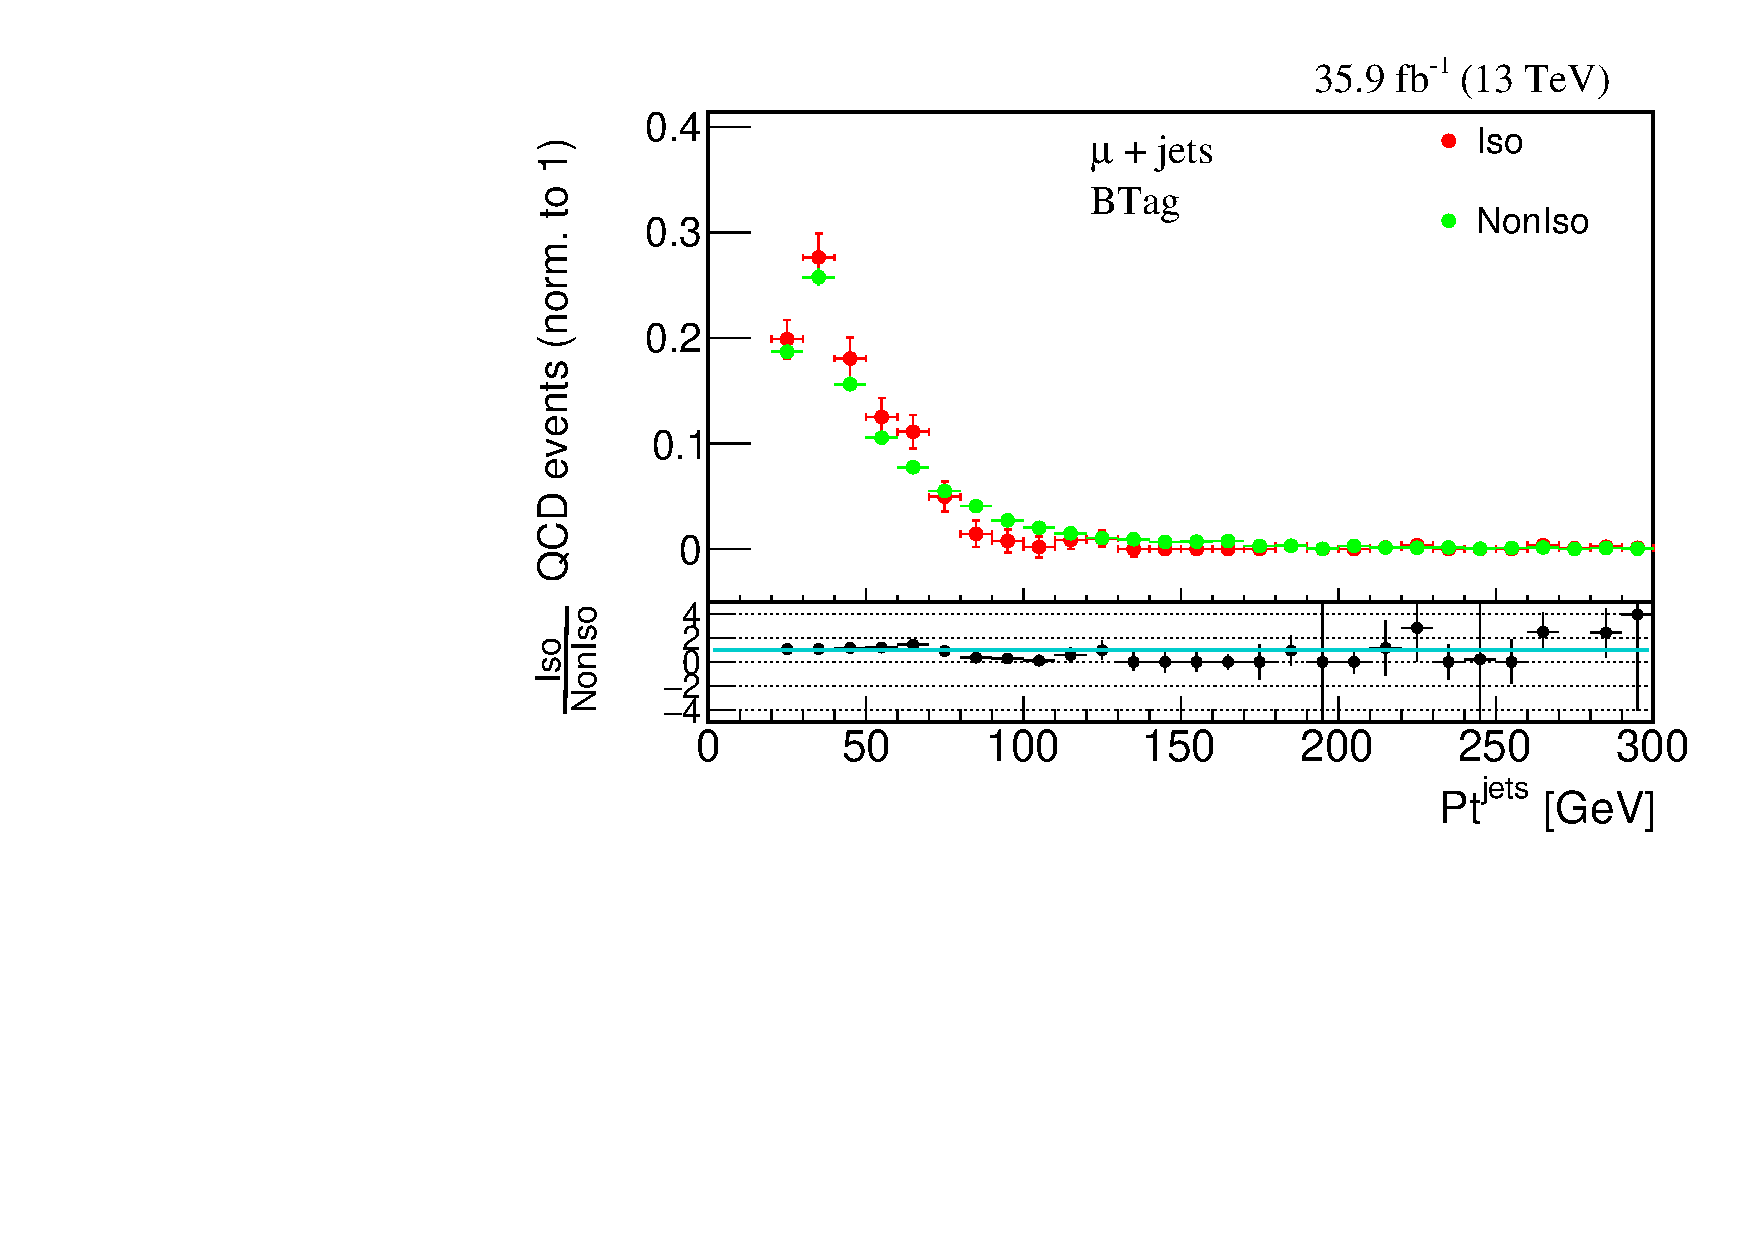
\includegraphics[width=0.40\linewidth]{Image/Muon/QCD/mu_BTag_pt_jet.pdf}}
    \subfigure[$\pt$ of jets \label{subfig:ele_BTag_pt_jet.pdf}]
    {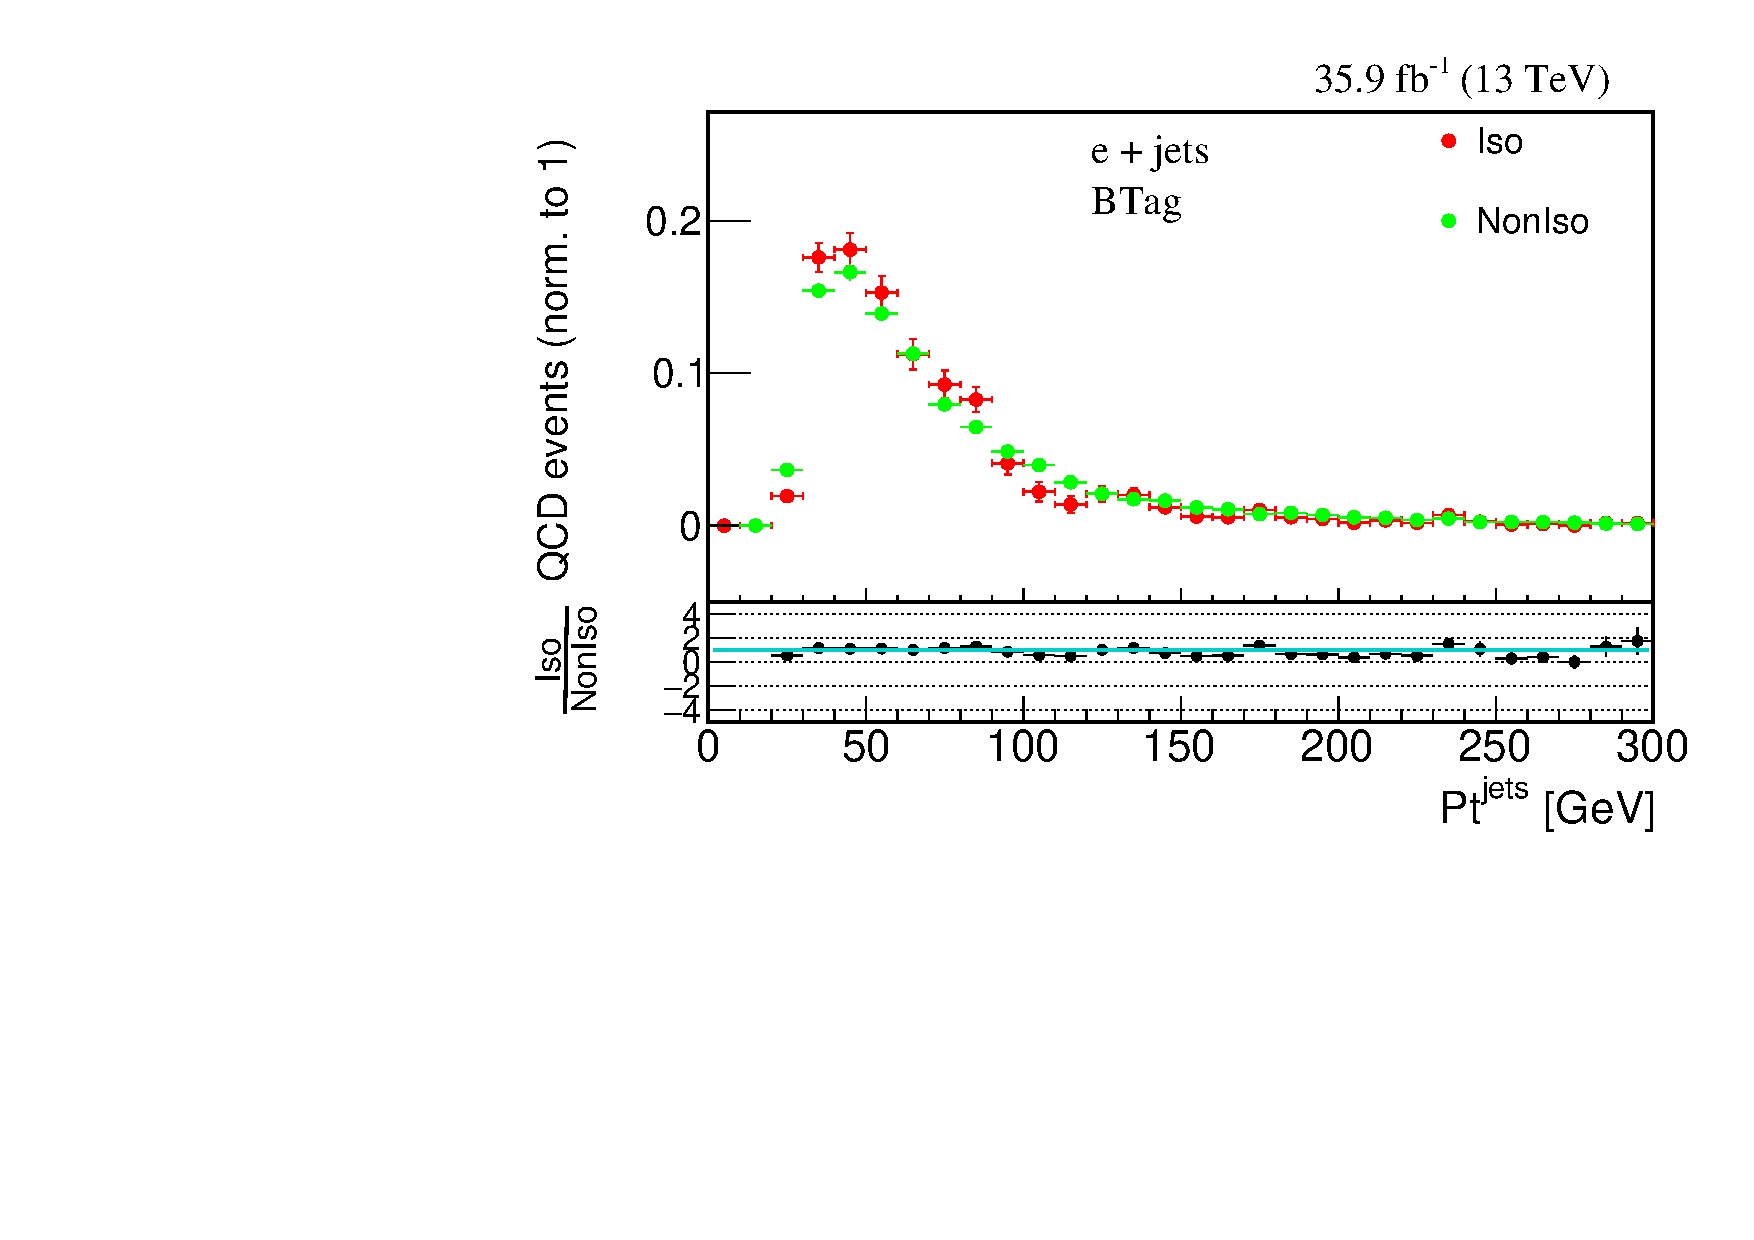
\includegraphics[width=0.40\linewidth]{Image/Electron/QCD/ele_BTag_pt_jet.pdf}}
    \caption{Comparison of data-driven QCD multijet shapes in low \MET region ($< 20$ \GeV), from
    the isolated and anti-isolated region with reconstructed jets after \PQb jet selection for \mujets 	   and \ejets channel.}
    \label{fig:qcd_shape_btag}
\end{figure}

\begin{figure}
    \centering  
    \subfigure[$\eta$ of muon \label{subfig:mu_KinFit_eta_mu.pdf}]
    {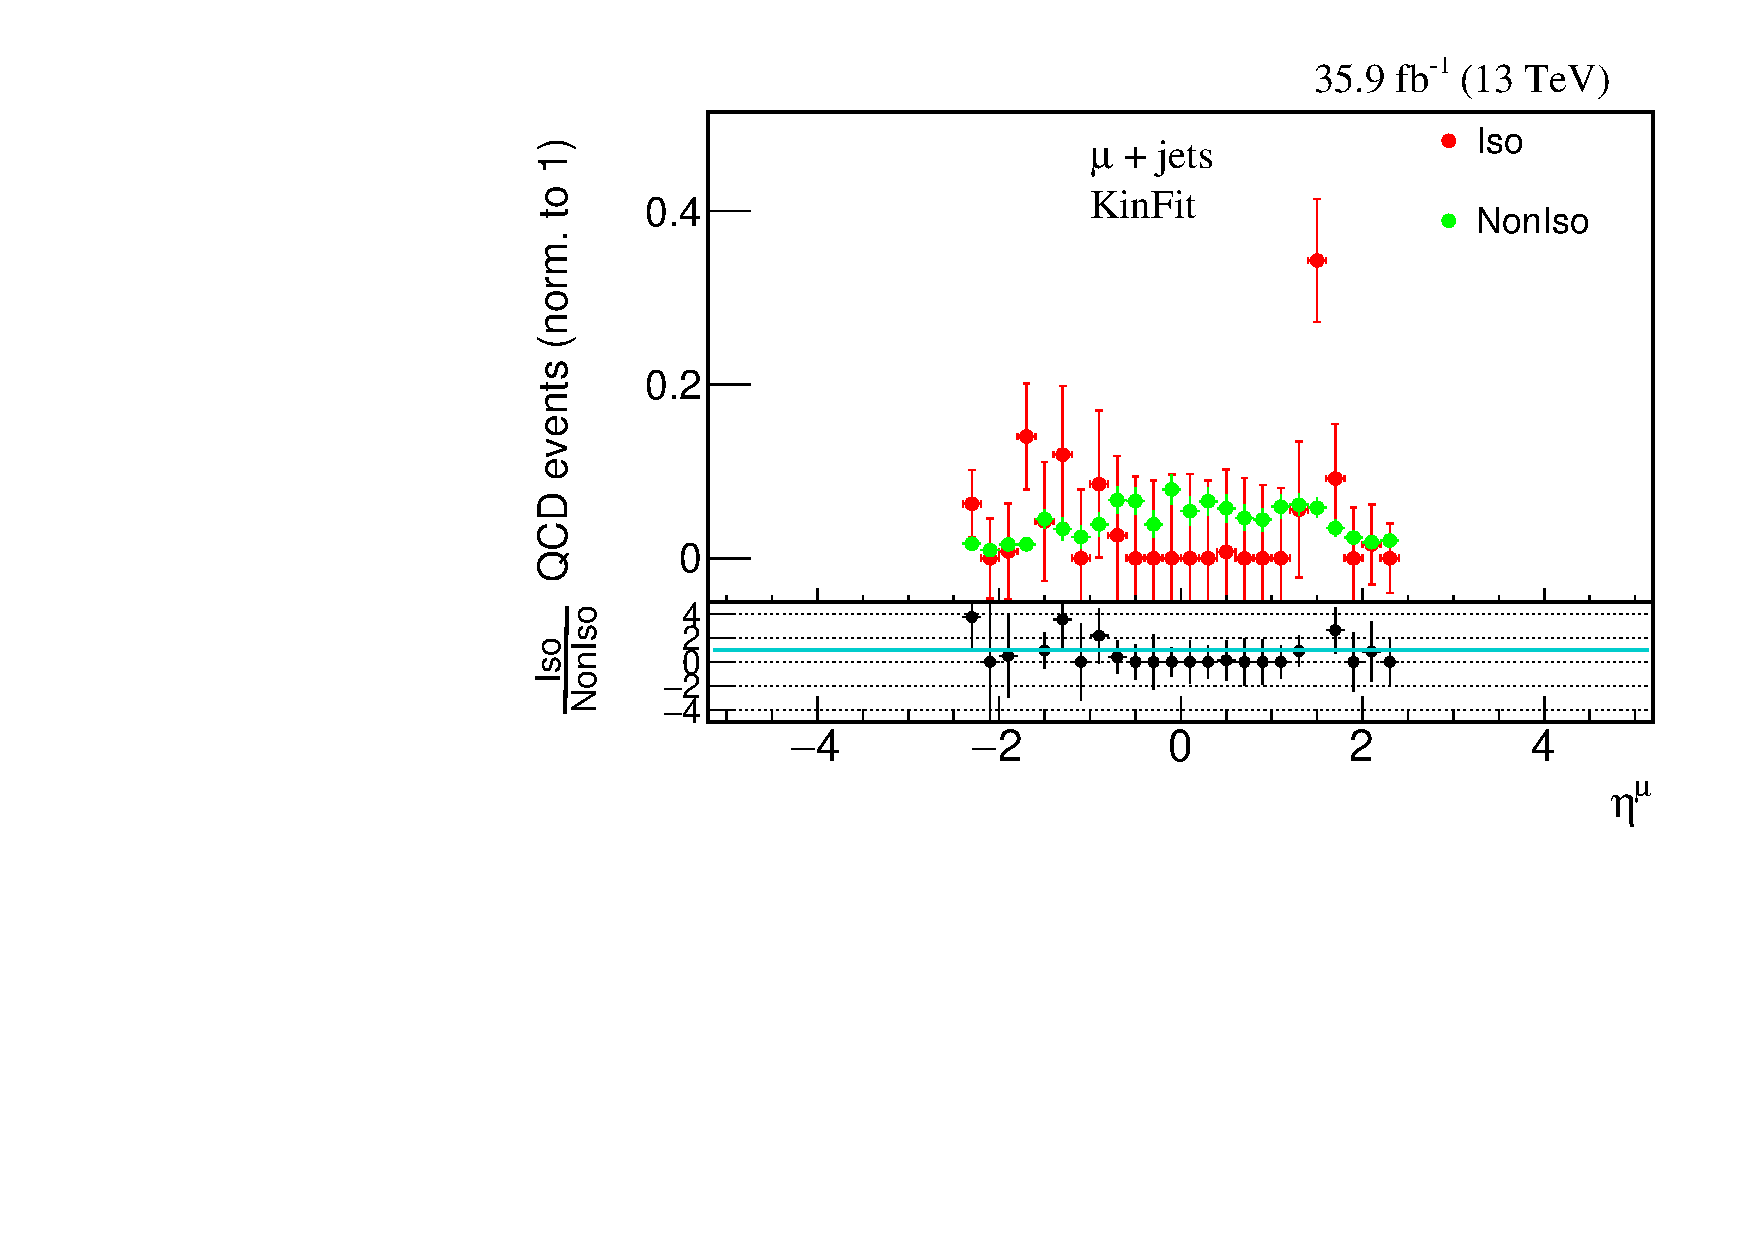
\includegraphics[width=0.40\linewidth]{Image/Muon/QCD/mu_KinFit_eta_mu.pdf}}
    \subfigure[$\eta$ of electron \label{subfig:ele_KinFit_eta_ele.pdf}]
    {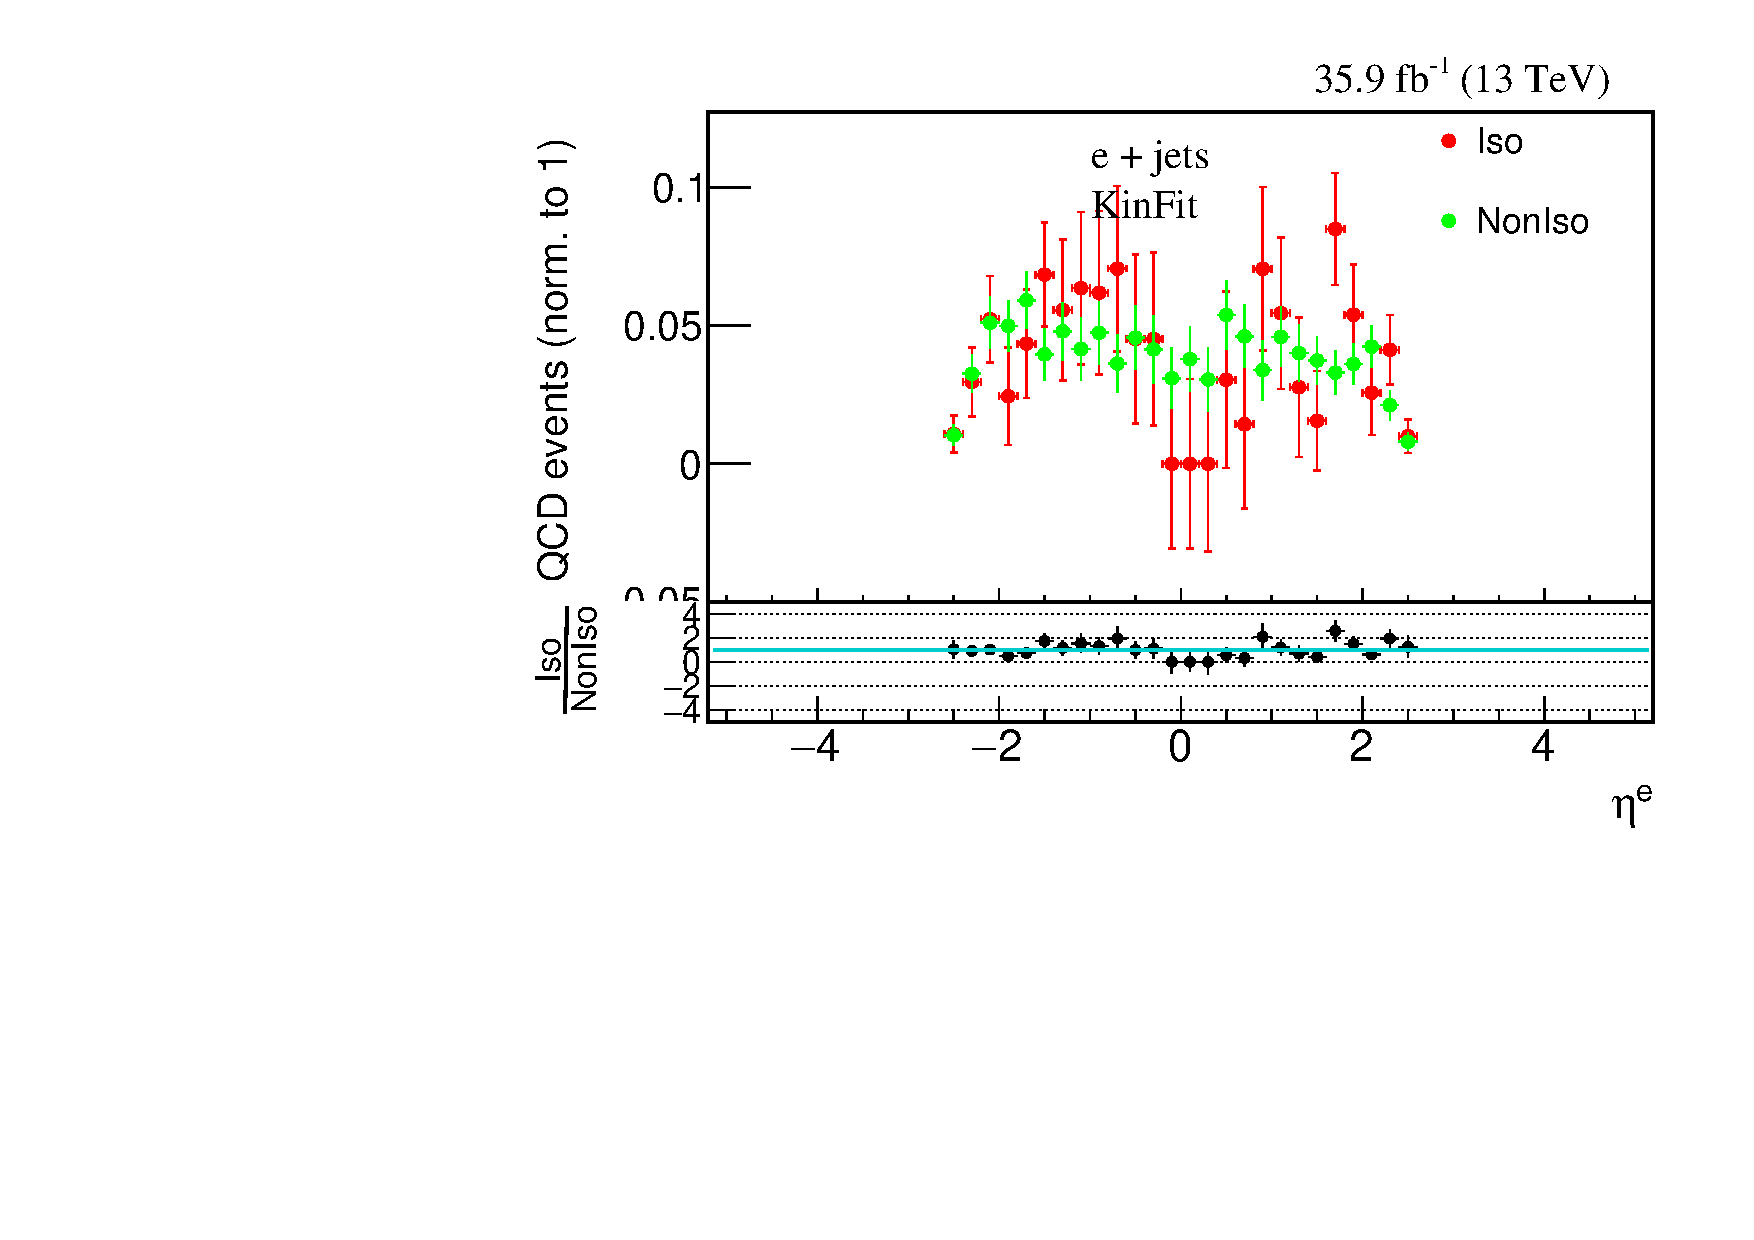
\includegraphics[width=0.40\linewidth]{Image/Electron/QCD/ele_KinFit_eta_ele.pdf}}
    \vfil
    \subfigure[$\eta$ of jets \label{subfig:mu_KinFit_eta_jet.pdf}]
    {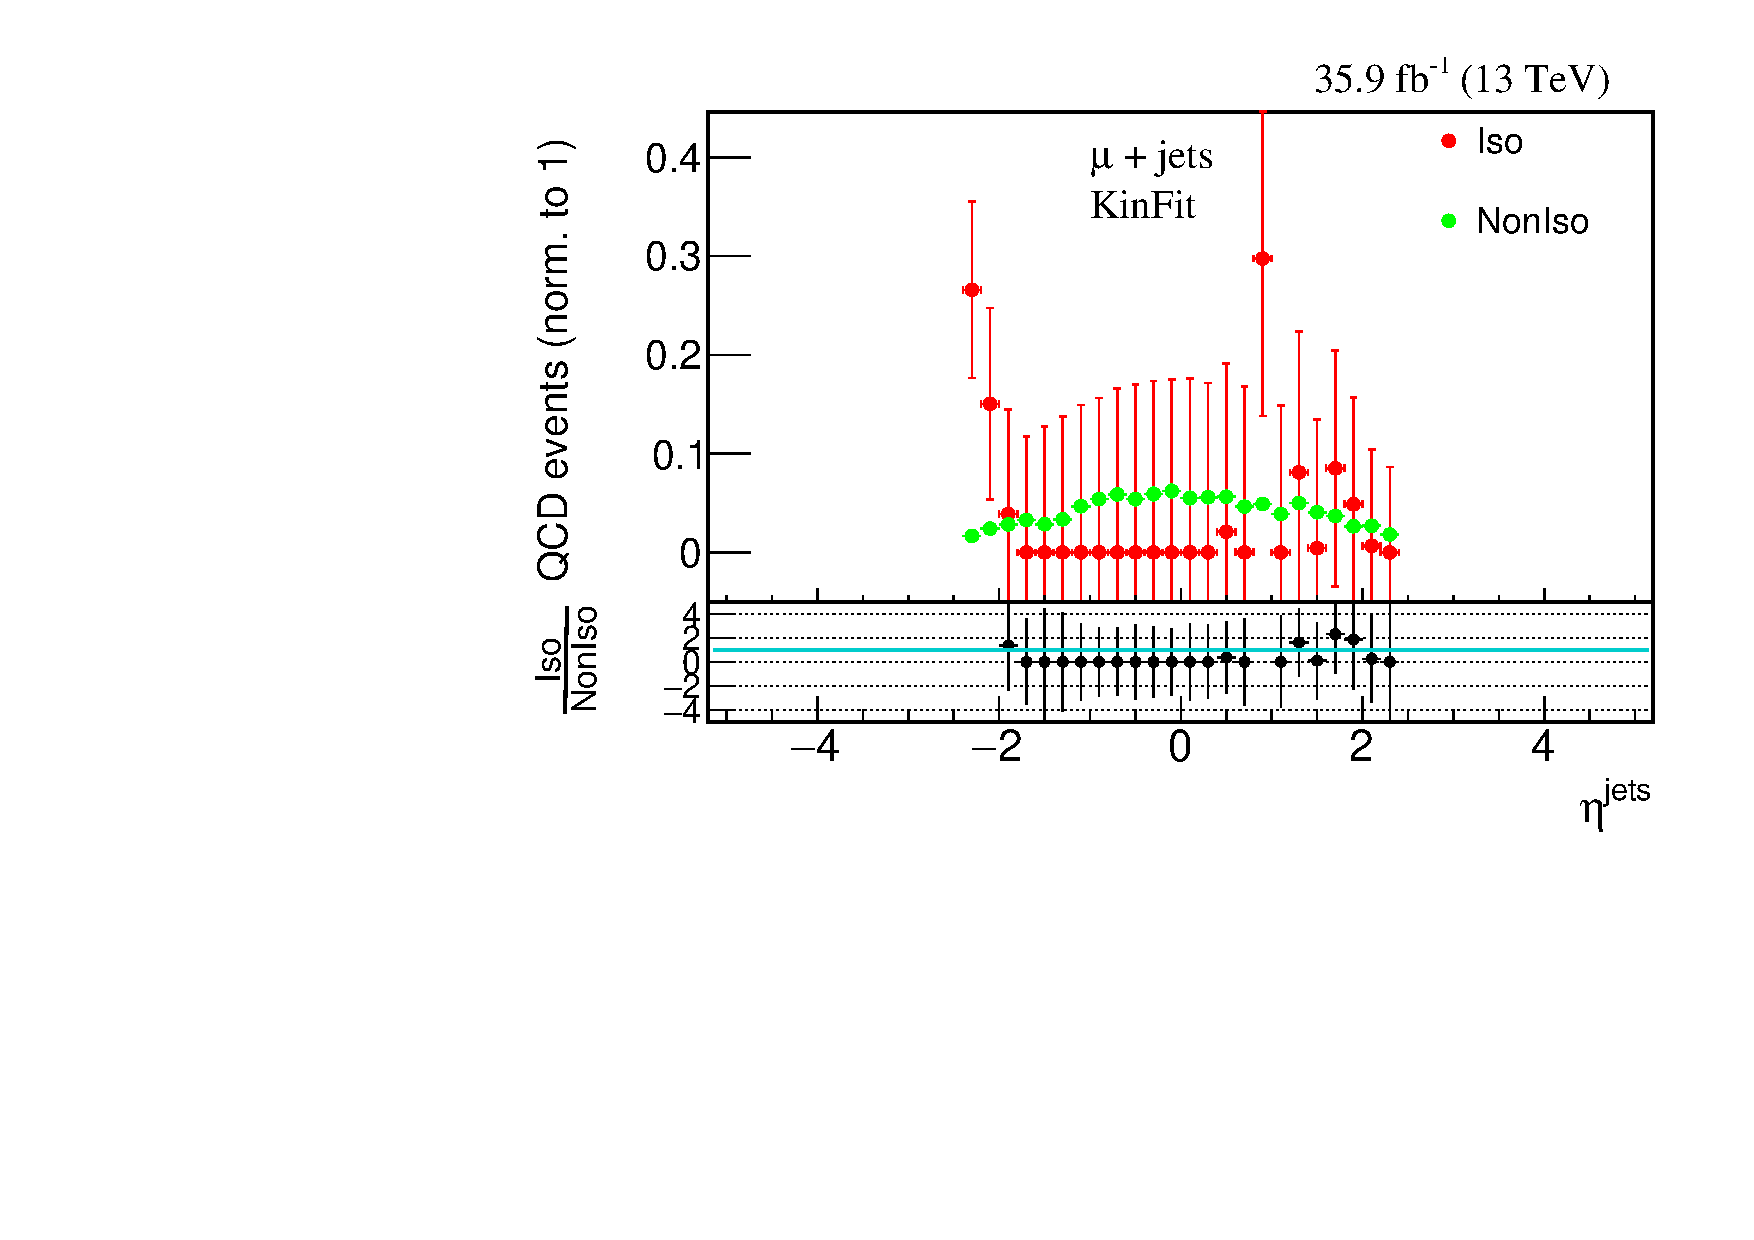
\includegraphics[width=0.40\linewidth]{Image/Muon/QCD/mu_KinFit_eta_jet.pdf}}
    \subfigure[$\eta$ of jets \label{subfig:ele_KinFit_eta_jet.pdf}]
    {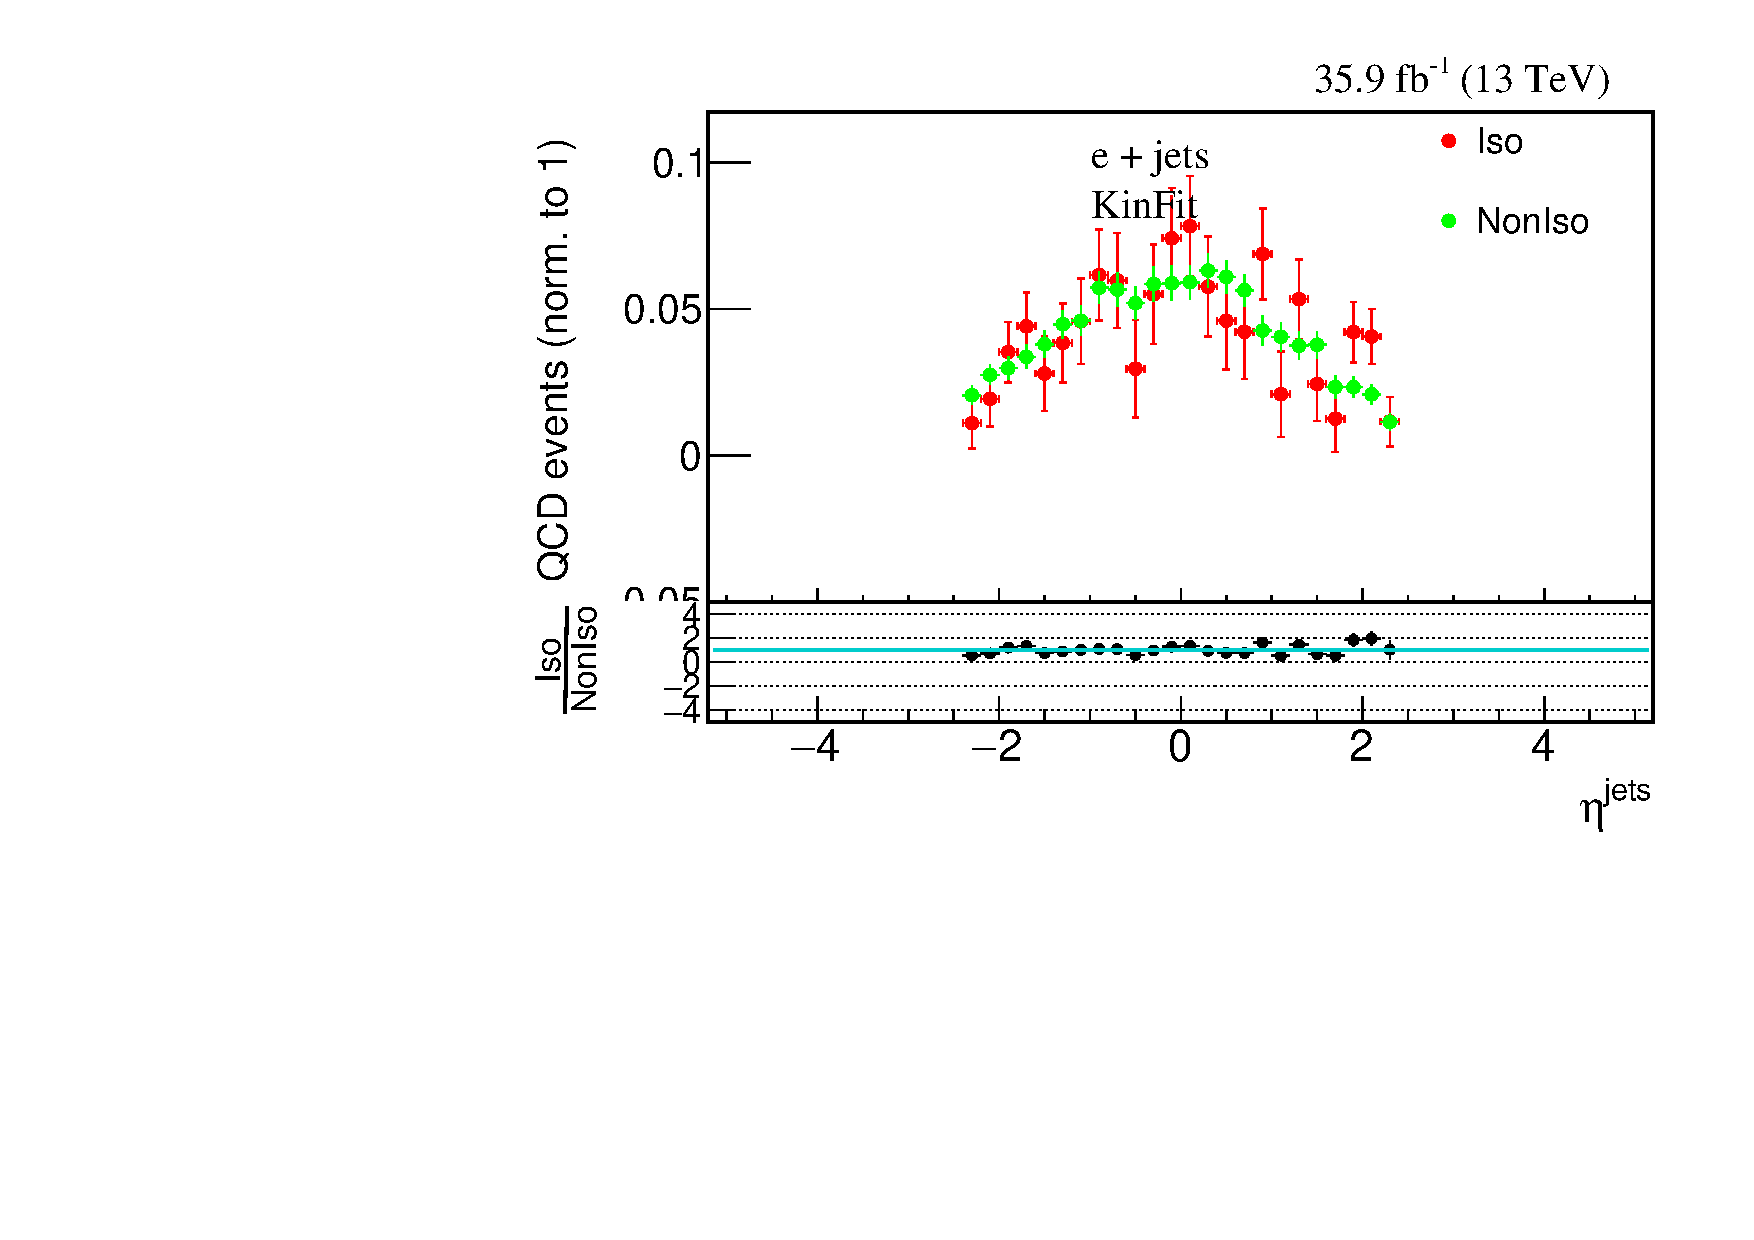
\includegraphics[width=0.40\linewidth]{Image/Electron/QCD/ele_KinFit_eta_jet.pdf}}
    \vfil
    \subfigure[$\pt$ of muon \label{subfig:mu_KinFit_pt_mu.pdf}]
    {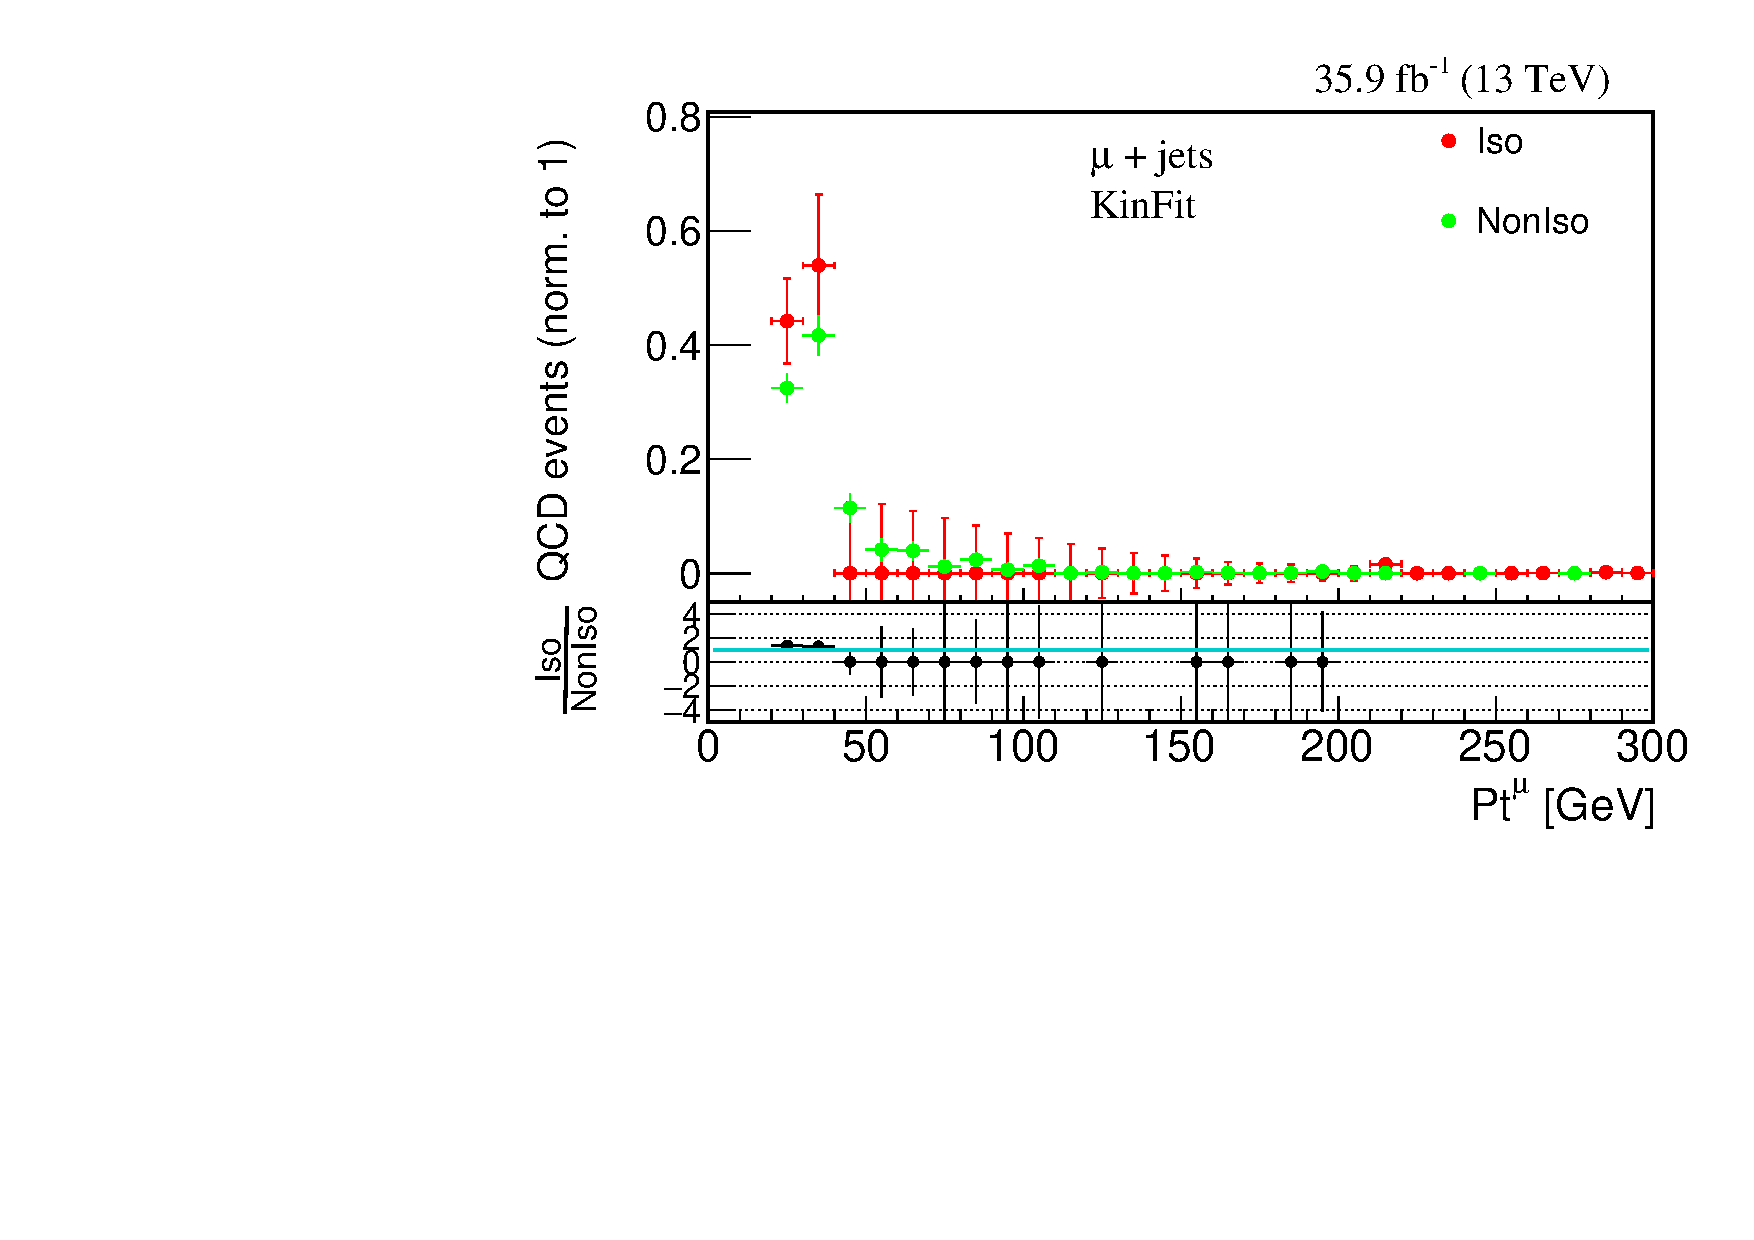
\includegraphics[width=0.40\linewidth]{Image/Muon/QCD/mu_KinFit_pt_mu.pdf}}
    \subfigure[$\pt$ of electron \label{subfig:ele_KinFit_pt_ele.pdf}]
    {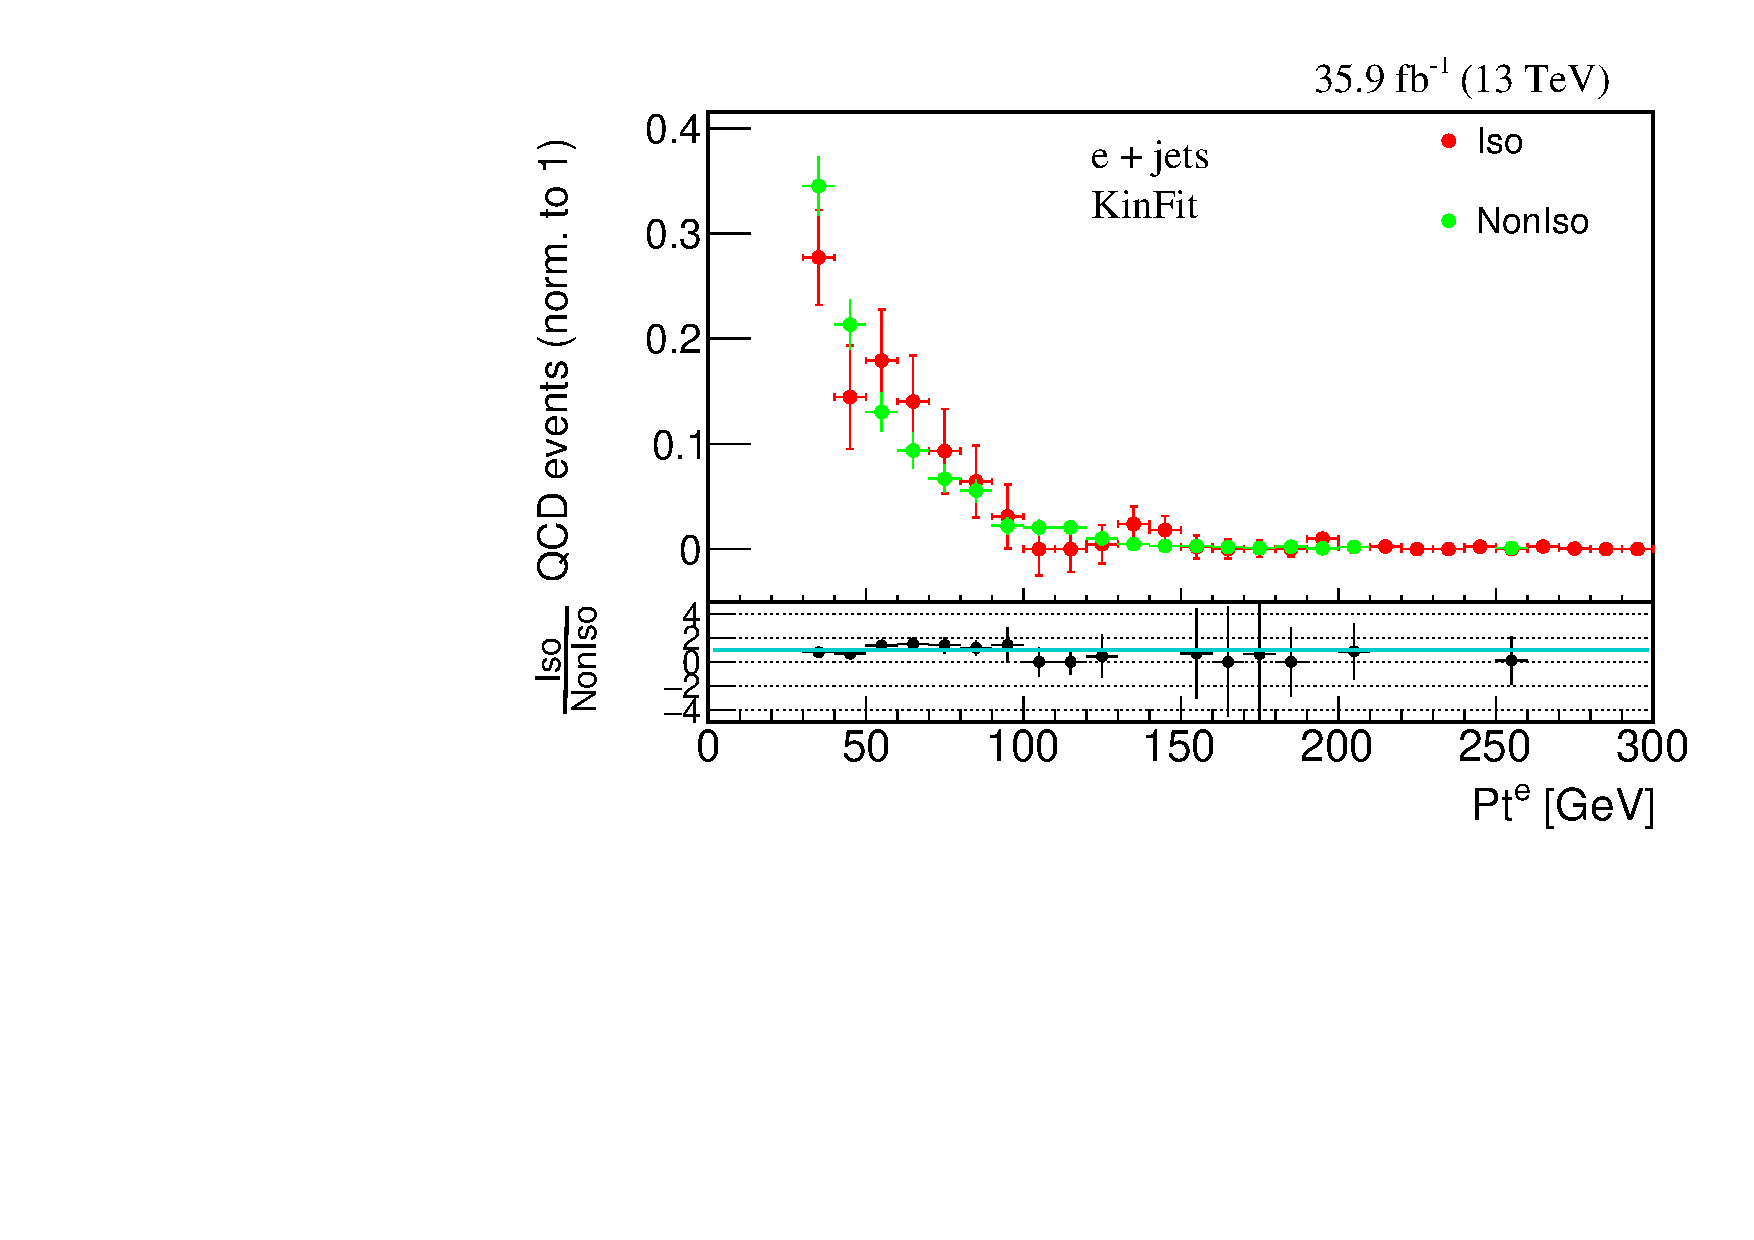
\includegraphics[width=0.40\linewidth]{Image/Electron/QCD/ele_KinFit_pt_ele.pdf}}
    \vfil
    \subfigure[$\pt$ of jets \label{subfig:mu_KinFit_pt_jet.pdf}]
    {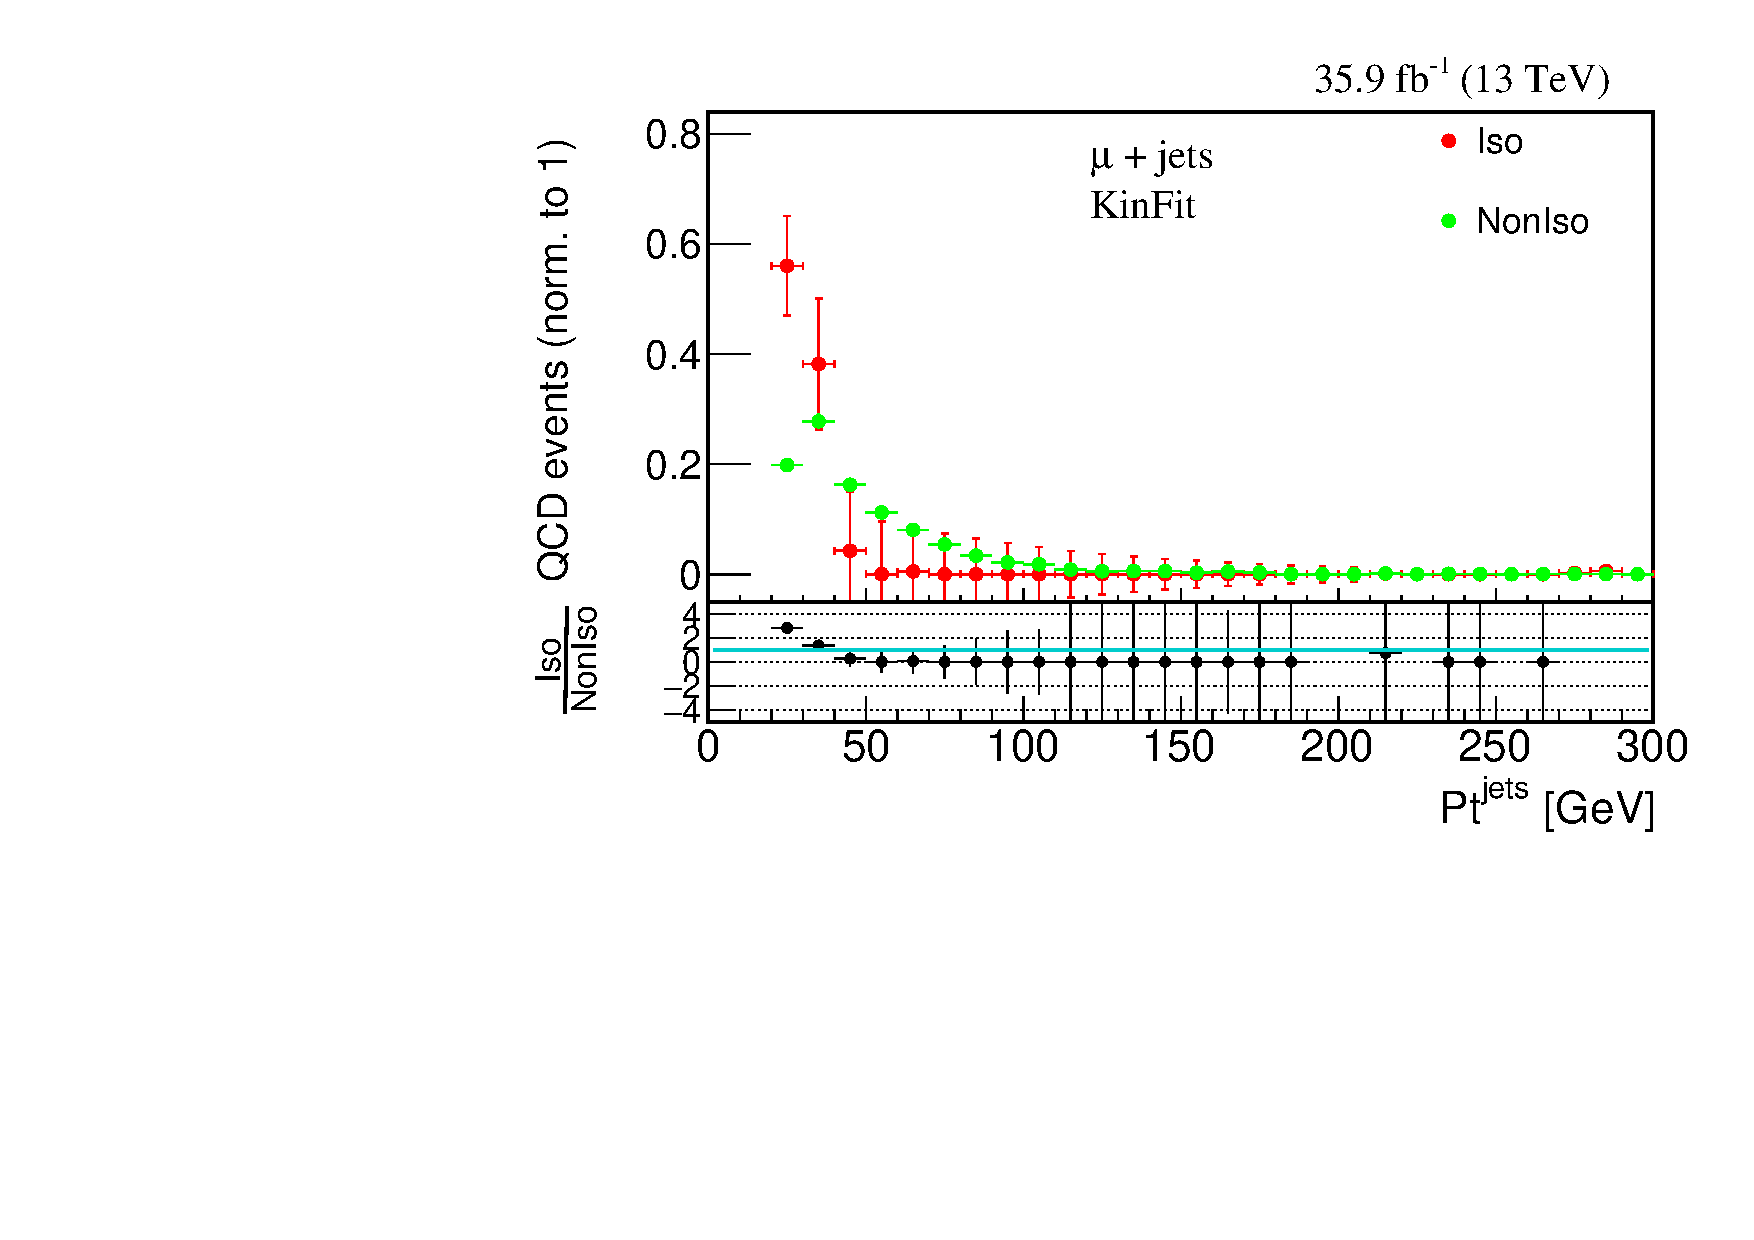
\includegraphics[width=0.40\linewidth]{Image/Muon/QCD/mu_KinFit_pt_jet.pdf}}
    \subfigure[$\pt$ of jets \label{subfig:ele_KinFit_pt_jet.pdf}]
    {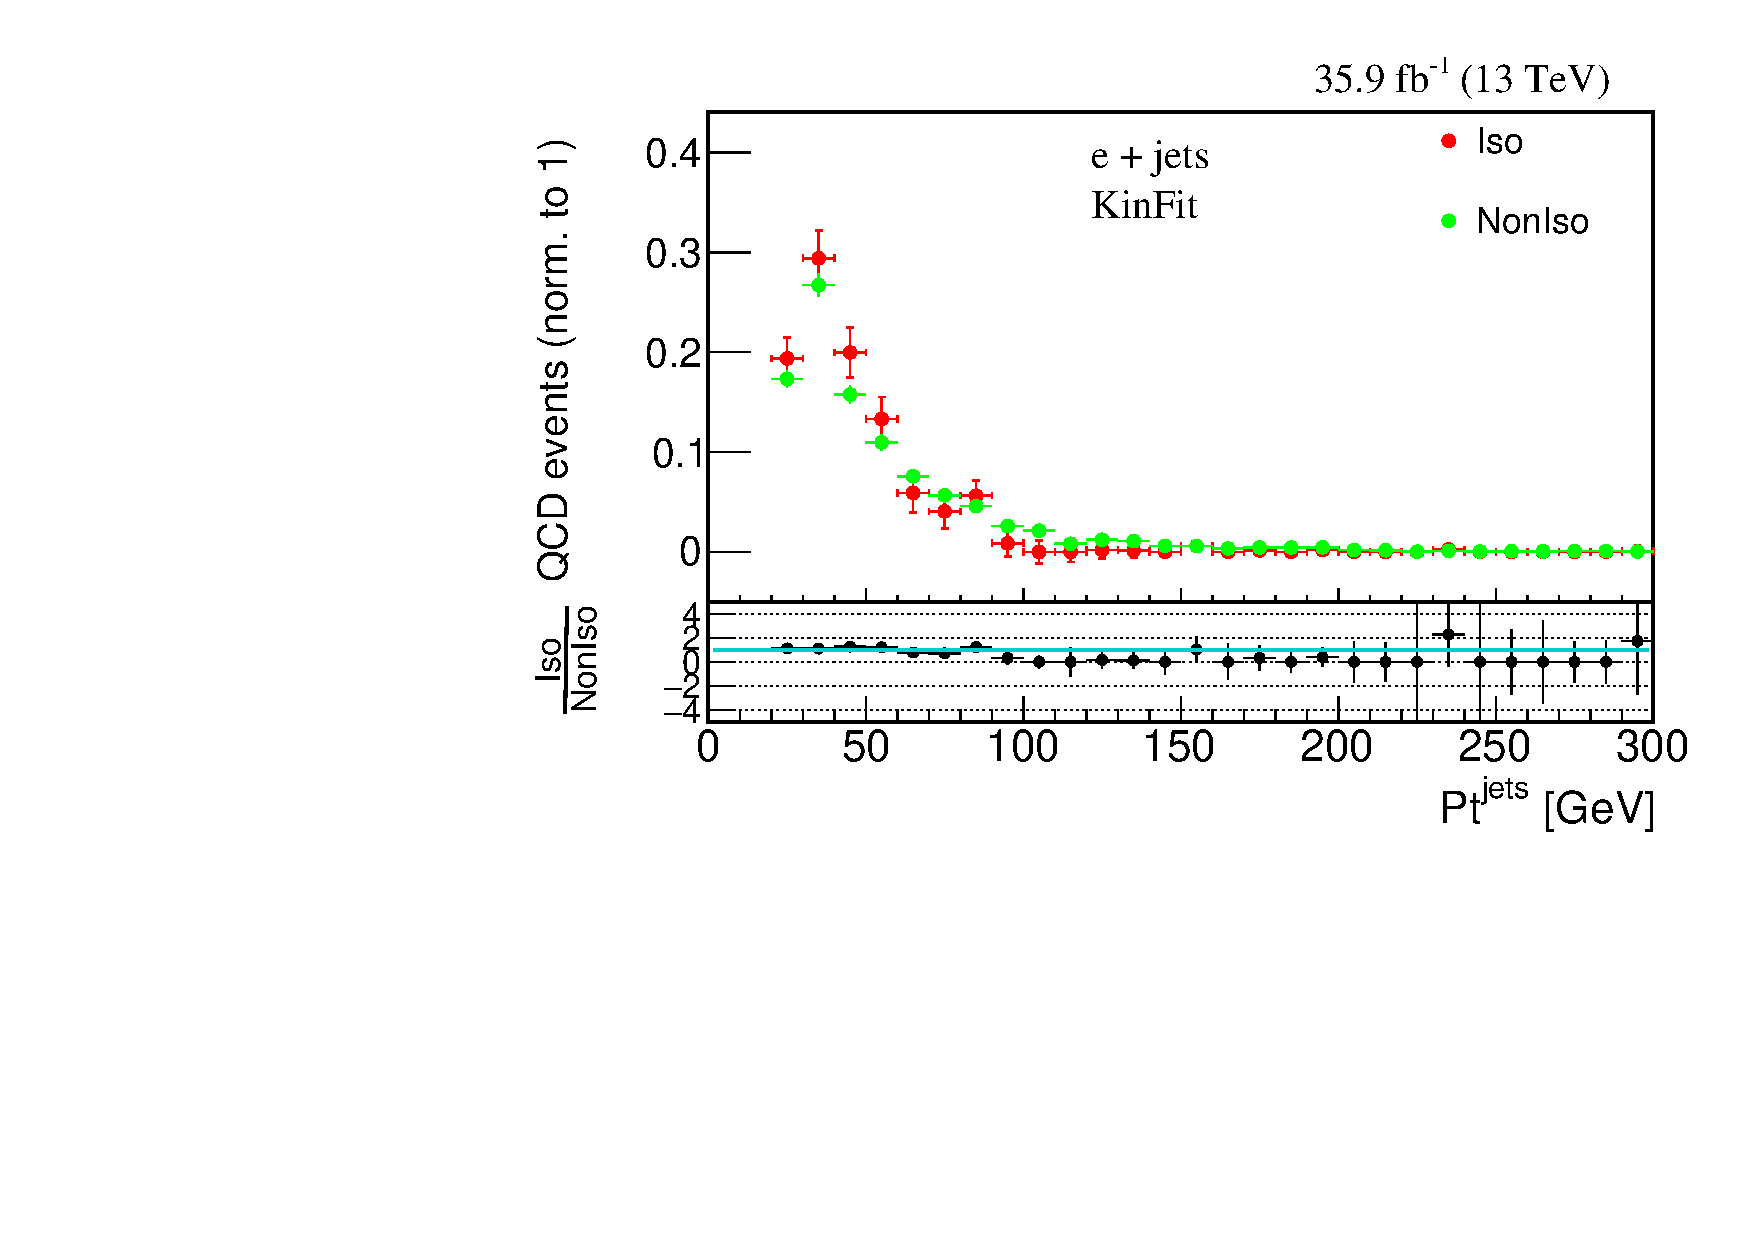
\includegraphics[width=0.40\linewidth]{Image/Electron/QCD/ele_KinFit_pt_jet.pdf}}
    \caption{Comparison of data-driven QCD multijet shapes in low \MET region ($ < 20$ \GeV), from 
	the isolated and anti-isolated region with kinematic fitted objects after kinematic fit 
	selection for \mujets and \ejets channel.}
    \label{fig:qcd_shape_kinfit}
\end{figure}

